% Формат А4, 14pt (ГОСТ Р 7.0.11-2011, 5.3.6)
\documentclass[a4paper,14pt]{extreport}

%%%%%%%%%%%%%%%%%%%%%%%%%%%%%%%%%%%%%%%%%%%%%%%%%%%%%%
%%%% Файл упрощённых настроек шаблона диссертации %%%%
%%%%%%%%%%%%%%%%%%%%%%%%%%%%%%%%%%%%%%%%%%%%%%%%%%%%%%

%%%        Подключение пакетов                 %%%
\usepackage{ifthen}                 % добавляет ifthenelse
%%% Инициализирование переменных, не трогать!  %%%
\newcounter{bibliosel}
%%%%%%%%%%%%%%%%%%%%%%%%%%%%%%%%%%%%%%%%%%%%%%%%%%

%%% Область упрощённого управления оформлением %%%

%% Библиография
\setcounter{bibliosel}{0}           % 0 --- встроенная реализация с загрузкой файла через движок bibtex8; 1 --- реализация пакетом biblatex через движок biber
               % Упрощённые настройки шаблона 

%%% Проверка используемого TeX-движка %%%
\usepackage{iftex}
\newif\ifxetexorluatex   % определяем новый условный оператор (http://tex.stackexchange.com/a/47579/79756)
\ifXeTeX
    \xetexorluatextrue
\else
    \ifLuaTeX
        \xetexorluatextrue
    \else
        \xetexorluatexfalse
    \fi
\fi

%%% Поля и разметка страницы %%%
\usepackage{pdflscape}                              % Для включения альбомных страниц
\usepackage{geometry}                               % Для последующего задания полей

%%% Математические пакеты %%%
\usepackage{amsthm,amsfonts,amsmath,amssymb,amscd}  % Математические дополнения от AMS
\usepackage{mathtools}                              % Добавляет окружение multlined

%%%% Установки для размера шрифта 14 pt %%%%
%% Формирование переменных и констант для сравнения (один раз для всех подключаемых файлов)%%
%% должно располагаться до вызова пакета fontspec или polyglossia, потому что они сбивают его работу
\newlength{\curtextsize}
\newlength{\bigtextsize}
\setlength{\bigtextsize}{13.9pt}

\makeatletter
%\show\f@size                                       % неплохо для отслеживания, но вызывает стопорение процесса, если документ компилируется без команды  -interaction=nonstopmode 
\setlength{\curtextsize}{\f@size pt}
\makeatother

%%% Кодировки и шрифты %%%
\ifxetexorluatex
    \usepackage{polyglossia}                        % Поддержка многоязычности (fontspec подгружается автоматически)
\else
    \RequirePDFTeX                                  % tests for PDFTEX use and throws an error if a different engine is being used
    \usepackage{cmap}                               % Улучшенный поиск русских слов в полученном pdf-файле
    \usepackage[T2A]{fontenc}                       % Поддержка русских букв
    \usepackage[utf8]{inputenc}                     % Кодировка utf8
    \usepackage[english, russian]{babel}            % Языки: русский, английский
    \IfFileExists{pscyr.sty}{\usepackage{pscyr}}{}  % Красивые русские шрифты
\fi

%%% Оформление абзацев %%%
\usepackage{indentfirst}                            % Красная строка

%%% Цвета %%%
\usepackage[dvipsnames,usenames]{color}
\usepackage{colortbl}

%%% Таблицы %%%
\usepackage{longtable}                              % Длинные таблицы
\usepackage{multirow,makecell,array}                % Улучшенное форматирование таблиц
\usepackage{booktabs}                               % Возможность оформления таблиц в классическом книжном стиле (при правильном использовании не противоречит ГОСТ)

%%% Общее форматирование
\usepackage{soulutf8}                               % Поддержка переносоустойчивых подчёркиваний и зачёркиваний
\usepackage{icomma}                                 % Запятая в десятичных дробях


%%% Гиперссылки %%%
\usepackage{hyperref}

%%% Изображения %%%
\usepackage{graphicx}                               % Подключаем пакет работы с графикой

%%% Списки %%%
\usepackage[cache=false]{minted}
\usepackage{enumitem}

%%% Подписи %%%
\usepackage{caption}                                % Для управления подписями (рисунков и таблиц) % Может управлять номерами рисунков и таблиц с caption %Иногда может управлять заголовками в списках рисунков и таблиц
\usepackage{subcaption}                             % Работа с подрисунками и подобным

%%% Интервалы %%%
\usepackage[onehalfspacing]{setspace}               % Опция запуска пакета правит не только интервалы в обычном тексте, но и формульные

%%% Счётчики %%%
\usepackage[figure,table]{totalcount}               % Счётчик рисунков и таблиц
\usepackage{totcount}                               % Пакет создания счётчиков на основе последнего номера подсчитываемого элемента (может требовать дважды компилировать документ)
\usepackage{totpages}                               % Счётчик страниц, совместимый с hyperref (ссылается на номер последней страницы). Желательно ставить последним пакетом в преамбуле  % Пакеты общие для диссертации и автореферата
%%% Колонтитулы %%%
\usepackage{fancyhdr}

%%% Прикладные пакеты %%% 
\usepackage{calc}               % Пакет для расчётов параметров, например длины
%\usepackage{etoolbox}          % ради функции patchcmd для управления списком литературы

\usepackage {interfaces-base}   % Набор базовых интерфейсов к некоторым пакетам, конкретные реализации загружаются в стиле

%%% Заголовки %%%
\usepackage{titlesec}           % Пакет настройки шрифтов заголовков в тексте

%%% Оглавление %%%
\usepackage{tocloft}

%%% Счётчики %%%
\usepackage{chngcntr}           % оперативная перенастройка счётчиков         % Пакеты для диссертации
\usepackage{tabularx,tabulary}  %таблицы с автоматически подбирающейся шириной столбцов

% Листинги с исходным кодом программ
\usepackage{fancyvrb}
\usepackage{listings}

% Плавающие окружения. во многом лучше пакета float
\usepackage{floatrow}
        % Пакеты для специфических пользовательских задач
%%% Переопределение именований, чтобы можно было и в преамбуле использовать %%%
\renewcommand{\chaptername}{Глава}
\renewcommand{\appendixname}{Приложение} % (ГОСТ Р 7.0.11-2011, 5.7)
       % Переопределение именований, чтобы можно было и в преамбуле использовать
%%% Макет страницы %%%
% Выставляем значения полей (ГОСТ 7.0.11-2011, 5.3.7)
\geometry{a4paper,top=2cm,bottom=2cm,left=2.5cm,right=1cm}

%%% Кодировки и шрифты %%%
\ifxetexorluatex
    \setmainlanguage[babelshorthands=true]{russian}  % Язык по-умолчанию русский с поддержкой приятных команд пакета babel
    \setotherlanguage{english}                       % Дополнительный язык = английский (в американской вариации по-умолчанию)
    \ifXeTeX
        \defaultfontfeatures{Ligatures=TeX,Mapping=tex-text}
    \else
        \defaultfontfeatures{Ligatures=TeX}
    \fi
    \setmainfont{Times New Roman}
    \newfontfamily\cyrillicfont{Times New Roman}
    \setsansfont{Arial}
    \newfontfamily\cyrillicfontsf{Arial}
    \setmonofont{Courier New}
    \newfontfamily\cyrillicfonttt{Courier New}
\else
    \IfFileExists{pscyr.sty}{\renewcommand{\rmdefault}{ftm}}{}
\fi

%%% Интервалы %%%
%linespread-реализация ближе к реализации полуторного интервала в ворде.
%setspace реализация заточена под шрифты 10, 11, 12pt, под остальные кегли хуже, но всё же ближе к типографской классике. 
%\linespread{1.3}                    % Полуторный интервал (ГОСТ Р 7.0.11-2011, 5.3.6)

%%% Выравнивание и переносы %%%
\sloppy                             % Избавляемся от переполнений
\clubpenalty=10000                  % Запрещаем разрыв страницы после первой строки абзаца
\widowpenalty=10000                 % Запрещаем разрыв страницы после последней строки абзаца

%%% Изображения %%%
\graphicspath{{images/}}            % Пути к изображениям

%%% Подписи %%%
\captionsetup{%
singlelinecheck=off,                % Многострочные подписи, например у таблиц
skip=2pt,                           % Вертикальная отбивка между подписью и содержимым рисунка или таблицы определяется ключом
justification=centering,            % Центрирование подписей, заданных командой \caption
}

%%% Рисунки %%%
\DeclareCaptionLabelSeparator*{emdash}{~--- }             % (ГОСТ 2.105, 4.3.1)
\captionsetup[figure]{labelsep=emdash,font=onehalfspacing,position=bottom}

%%% Таблицы %%%
\DeclareCaptionFormat{tablecaption}{\raggedleft #1#2\\%   % Идентификатор таблицы справа, на отдельной строке
    \centering{#3}}                                       % Наименование таблицы строкой ниже и центрировано, без переносов
\DeclareCaptionFormat{tablenocaption}{\raggedleft #1#2%   % Идентификатор таблицы справа, на отдельной строке
}                                                         % Наименование таблицы отсутствует
\captionsetup[table]{format=tablecaption,labelsep=space,singlelinecheck=off,font=onehalfspacing,position=top}  % пробельный разделитьель идентификатора с номером от наименования, многострочные наименования и прочее
\DeclareCaptionLabelFormat{continued}{Продолжение таблицы~#2}

%%% Подписи подрисунков %%%
\renewcommand{\thesubfigure}{\asbuk{subfigure}}           % Буквенные номера подрисунков
\captionsetup[subfigure]{font={normalsize},               % Шрифт подписи названий подрисунков (не отличается от основного)
    labelformat=brace,                                    % Формат обозначения подрисунка
    justification=centering,                              % Выключка подписей (форматирование), один из вариантов            
}
%\DeclareCaptionFont{font12pt}{\fontsize{12pt}{13pt}\selectfont} % объявляем шрифт 12pt для использования в подписях, тут же надо интерлиньяж объявлять, если не наследуется
%\captionsetup[subfigure]{font={font12pt}}                 % Шрифт подписи названий подрисунков (всегда 12pt)

%%% Цвета гиперссылок %%%
\definecolor{linkcolor}{rgb}{0.9,0,0}
\definecolor{citecolor}{rgb}{0,0.6,0}
\definecolor{urlcolor}{rgb}{0,0,1}

%%% Настройки гиперссылок %%%
\hypersetup{
    linktocpage=true,           % ссылки с номера страницы в оглавлении, списке таблиц и списке рисунков
%    pdfpagelabels=false,        % set PDF page labels (true|false)
    plainpages=false,           % Forces page anchors to be named by the Arabic form  of the page number, rather than the formatted form
    colorlinks,                 % ссылки отображаются раскрашенным текстом, а не раскрашенным прямоугольником, вокруг текста
    linkcolor={linkcolor},      % цвет ссылок типа ref, eqref и подобных
    citecolor={citecolor},      % цвет ссылок-цитат
    urlcolor={urlcolor},        % цвет гиперссылок
}

\ifLuaTeX
    \hypersetup{
        unicode,                % Unicode encoded PDF strings
    }
\fi

%%% Шаблон %%%
\DeclareRobustCommand{\todo}{\textcolor{red}}       % решаем проблему превращения названия цвета в результате \MakeUppercase, http://tex.stackexchange.com/a/187930/79756 , \DeclareRobustCommand protects \todo from expanding inside \MakeUppercase
\setlength{\parindent}{2.5em}                       % Абзацный отступ. Должен быть одинаковым по всему тексту и равен пяти знакам (ГОСТ Р 7.0.11-2011, 5.3.7).

%%% Списки %%%
% Используем дефис для ненумерованных списков (ГОСТ 2.105-95, 4.1.7)
\renewcommand{\labelitemi}{\normalfont\bfseries{--}} 
\setlist{nosep,%                                    % Единый стиль для всех списков (пакет enumitem), без дополнительных интервалов.
    labelindent=\parindent,leftmargin=*%            % Каждый пункт, подпункт и перечисление записывают с абзацного отступа (ГОСТ 2.105-95, 4.1.8)
}
    % Стили общие для диссертации и автореферата
\LoadInterface {titlesec}                   % Подгружаем интерфейсы для дополнительных опций управления некоторыми пакетами

%%% Блок управления параметрами для выравнивания заголовков в тексте %%%
\newlength{\otstuplen}
\setlength{\otstuplen}{\theotstup\parindent}
\ifthenelse{\equal{\theheadingalign}{0}}{% выравнивание заголовков в тексте
    \newcommand{\hdngalign}{\filcenter}                % по центру
    \newcommand{\hdngaligni}{\hfill\hspace{\otstuplen}}% по центру
}{%
    \newcommand{\hdngalign}{\filright}                 % по левому краю
    \newcommand{\hdngaligni}{\hspace{\otstuplen}}      % по левому краю
} % В обоих случаях вроде бы без переноса, как и надо (ГОСТ Р 7.0.11-2011, 5.3.5)

%%% Оглавление %%%
\renewcommand{\cftchapdotsep}{\cftdotsep}                % отбивка точками до номера страницы начала главы/раздела
\renewcommand{\cfttoctitlefont}{\hdngaligni\fontsize{14pt}{16pt}\selectfont\bfseries}% вместе со следующей строкой
\renewcommand{\cftaftertoctitle}{\hfill}                 % устанавливает заголовок по центру
\setlength{\cftbeforetoctitleskip}{-1.4\curtextsize}     % Поскольку этот заголовок всегда является первым на странице, то перед ним отделять пустым тройным интервалом не следует. Независимо от основного шрифта, в этом случае зануление (почти) происходит при -1.4\curtextsize.
\setlength{\cftaftertoctitleskip}{\theintvl\curtextsize} % Если считаем Оглавление заголовком, то выставляем после него тройной интервал через наше определённое значение

%% Переносить слова в заголовке не допускается (ГОСТ Р 7.0.11-2011, 5.3.5). Заголовки в оглавлении должны точно повторять заголовки в тексте (ГОСТ Р 7.0.11-2011, 5.2.3). Прямого указания на запрет переносов в оглавлении нет, но по той же логике невнесения искажений в смысл, лучше в оглавлении не переносить:
\cftsetrmarg{2.55em plus1fil}                       %To have the (sectional) titles in the ToC, etc., typeset ragged right with no hyphenation
\renewcommand{\cftchappagefont}{\normalfont}        % нежирные номера страниц у глав в оглавлении
\renewcommand{\cftchapleader}{\cftdotfill{\cftchapdotsep}}% нежирные точки до номеров страниц у глав в оглавлении
%\renewcommand{\cftchapfont}{}                       % нежирные названия глав в оглавлении

\ifthenelse{\theheadingdelim > 0}{%
    \renewcommand\cftchapaftersnum{.\ }   % добавляет точку с пробелом после номера раздела в оглавлении
}{%
\renewcommand\cftchapaftersnum{\quad}     % добавляет \quad после номера раздела в оглавлении
}
\ifthenelse{\theheadingdelim > 1}{%
    \renewcommand\cftsecaftersnum{.\ }    % добавляет точку с пробелом после номера подраздела в оглавлении
    \renewcommand\cftsubsecaftersnum{.\ } % добавляет точку с пробелом после номера подподраздела в оглавлении
}{%
\renewcommand\cftsecaftersnum{\quad}      % добавляет \quad после номера подраздела в оглавлении
\renewcommand\cftsubsecaftersnum{\quad}   % добавляет \quad после номера подподраздела в оглавлении
}

\ifthenelse{\equal{\thepgnum}{1}}{%
    \addtocontents{toc}{~\hfill{Стр.}\par}% добавить Стр. над номерами страниц
}

%%% Оформление названий глав %%%
%% настройки заголовка списка рисунков
\renewcommand{\cftloftitlefont}{\hdngaligni\fontsize{14pt}{16pt}\selectfont\bfseries}% вместе со следующей строкой
\renewcommand{\cftafterloftitle}{\hfill}                                             % устанавливает заголовок по центру
\setlength{\cftbeforeloftitleskip}{-1.5\curtextsize}     % Поскольку этот заголовок всегда является первым на странице, то перед ним отделять пустым тройным интервалом не следует. Независимо от основного шрифта, в этом случае зануление (почти) происходит при -1.5\curtextsize.
\setlength{\cftafterloftitleskip}{\theintvl\curtextsize} % выставляем после него тройной интервал через наше определённое значение

%% настройки заголовка списка таблиц
\renewcommand{\cftlottitlefont}{\hdngaligni\fontsize{14pt}{16pt}\selectfont\bfseries}% вместе со следующей строкой
\renewcommand{\cftafterlottitle}{\hfill}                                             % устанавливает заголовок по центру
\setlength{\cftbeforelottitleskip}{-1.5\curtextsize}     % Поскольку этот заголовок всегда является первым на странице, то перед ним отделять пустым тройным интервалом не следует. Независимо от основного шрифта, в этом случае зануление (почти) происходит при -1.5\curtextsize.
\setlength{\cftafterlottitleskip}{\theintvl\curtextsize} % выставляем после него тройной интервал через наше определённое значение

\ifnum\curtextsize>\bigtextsize     % Проверяем условие использования базового шрифта 14 pt
\setlength{\headheight}{17pt}       % Исправляем высоту заголовка
\else
\setlength{\headheight}{15pt}       % Исправляем высоту заголовка
\fi

%%% Колонтитулы %%%
% Порядковый номер страницы печатают на середине верхнего поля страницы (ГОСТ Р 7.0.11-2011, 5.3.8)
\makeatletter
\let\ps@plain\ps@fancy              % Подчиняем первые страницы каждой главы общим правилам
\makeatother
\pagestyle{fancy}                   % Меняем стиль оформления страниц
\fancyhf{}                          % Очищаем текущие значения
\fancyhead[C]{\thepage}             % Печатаем номер страницы на середине верхнего поля
\renewcommand{\headrulewidth}{0pt}  % Убираем разделительную линию

%%% Оформление заголовков глав, разделов, подразделов %%%
%% Работа должна быть выполнена ... размером шрифта 12-14 пунктов (ГОСТ Р 7.0.11-2011, 5.3.8). То есть не должно быть надписей шрифтом более 14. Так и поставим.
%% Эти установки будут давать одинаковый результат независимо от выбора базовым шрифтом 12 пт или 14 пт
\titleformat{\chapter}[block]                                % default display;  hang = with a hanging label. (Like the standard \section.); block = typesets the whole title in a block (a paragraph) without additional formatting. Useful in centered titles
        {\hdngalign\fontsize{14pt}{16pt}\selectfont\bfseries}% 
        %\fontsize{<size>}{<skip>} % второе число ставим 1.2*первое, чтобы адекватно отрабатывали команды по расчету полуторного интервала (домножая разные комбинации коэффициентов на этот)
        {\thechapter\cftchapaftersnum}                       % Заголовки в оглавлении должны точно повторять заголовки в тексте (ГОСТ Р 7.0.11-2011, 5.2.3).
        {0em}% отступ от номера до текста
        {}%

\titleformat{\section}[block]                                % default hang;  hang = with a hanging label. (Like the standard \section.); block = typesets the whole title in a block (a paragraph) without additional formatting. Useful in centered titles
        {\hdngalign\fontsize{14pt}{16pt}\selectfont\bfseries}% 
        %\fontsize{<size>}{<skip>} % второе число ставим 1.2*первое, чтобы адекватно отрабатывали команды по расчету полуторного интервала (домножая разные комбинации коэффициентов на этот)
        {\thesection\cftsecaftersnum}                        % Заголовки в оглавлении должны точно повторять заголовки в тексте (ГОСТ Р 7.0.11-2011, 5.2.3).
        {0em}% отступ от номера до текста
        {}%

\titleformat{\subsection}[block]                             % default hang;  hang = with a hanging label. (Like the standard \section.); block = typesets the whole title in a block (a paragraph) without additional formatting. Useful in centered titles
        {\hdngalign\fontsize{14pt}{16pt}\selectfont\bfseries}% 
        %\fontsize{<size>}{<skip>} % второе число ставим 1.2*первое, чтобы адекватно отрабатывали команды по расчету полуторного интервала (домножая разные комбинации коэффициентов на этот)
        {\thesubsection\cftsubsecaftersnum}                  % Заголовки в оглавлении должны точно повторять заголовки в тексте (ГОСТ Р 7.0.11-2011, 5.2.3).
        {0em}% отступ от номера до текста
        {}%

\ifthenelse{\equal{\thechapstyle}{1}}{%
    \sectionformat{\chapter}{% Параметры заголовков разделов в тексте
        label=\chaptername\ \thechapter\cftchapaftersnum,
        labelsep=0em,
    }
    %% Следующие две строки: будет вписано слово Глава перед каждым номером раздела в оглавлении   
    \renewcommand{\cftchappresnum}{\chaptername\ }
    \setlength{\cftchapnumwidth}{\widthof{\cftchapfont\cftchappresnum\thechapter\cftchapaftersnum}}
}%

%% Интервалы между заголовками
% На эти величины titlespacing множит через *
\beforetitleunit=\curtextsize% привязались к нашему размеру шрифта
\aftertitleunit=\curtextsize% привязались к нашему размеру шрифта

% Счётчик intvl и длина \otstup определены в файле setup
\titlespacing{\chapter}{\theotstup\parindent}{-1.7em}{*\theintvl}       % Заголовки отделяют от текста сверху и снизу тремя интервалами (ГОСТ Р 7.0.11-2011, 5.3.5). Поскольку название главы всегда является первым на странице, то перед ним отделять пустым тройным интервалом не следует. Независимо от основного шрифта, в этом случае зануление происходит при -1.7em.
\titlespacing{\section}{\theotstup\parindent}{*\theintvl}{*\theintvl}
\titlespacing{\subsection}{\theotstup\parindent}{*\theintvl}{*\theintvl}
\titlespacing{\subsubsection}{\theotstup\parindent}{*\theintvl}{*\theintvl}

%%% Блок дополнительного управления размерами заголовков
\ifthenelse{\equal{\theheadingsize}{1}}{% Пропорциональные заголовки и базовый шрифт 14 пт
    \renewcommand{\cfttoctitlefont}{\hdngaligni\Large\bfseries} % Исправляем размер заголовка оглавления
    \setlength{\cftbeforetoctitleskip}{-1.2\curtextsize}        % Исправляем вертикальный отступ перед заголовком оглавления
    \renewcommand{\cftloftitlefont}{\hdngaligni\Large\bfseries} % Исправляем размер заголовка списка рисунков
    \setlength{\cftbeforeloftitleskip}{-1.4\curtextsize}        % Исправляем вертикальный отступ перед заголовком списка рисунков
    \renewcommand{\cftlottitlefont}{\hdngaligni\Large\bfseries} % Исправляем размер заголовка списка таблиц 
    \setlength{\cftbeforelottitleskip}{-1.4\curtextsize}        % Исправляем вертикальный отступ перед заголовком списка таблиц
    \sectionformat{\chapter}{% Параметры заголовков разделов в тексте
        format=\hdngalign\Large\bfseries, % Исправляем размер заголовка
        top-=0.4em,                       % Исправляем вертикальный отступ перед заголовком
    }
    \sectionformat{\section}{% Параметры заголовков подразделов в тексте
        format=\hdngalign\large\bfseries, % Исправляем размер заголовка
    }
}

\ifthenelse{\equal{\theheadingsize}{1}\AND \curtextsize < \bigtextsize}{% Пропорциональные заголовки и базовый шрифт 14 пт
    \sectionformat{\chapter}{% Параметры заголовков разделов в тексте
        top-=0.2em, % Исправляем вертикальный отступ перед заголовком
    }
}

%%% Счётчики %%%

%% Упрощённые настройки шаблона диссертации: нумерация формул, таблиц, рисунков
\ifthenelse{\equal{\thecontnum}{1}}{%
    \counterwithout{equation}{chapter} % Убираем связанность номера формулы с номером главы/раздела
    \counterwithout{figure}{chapter}   % Убираем связанность номера рисунка с номером главы/раздела
    \counterwithout{table}{chapter}    % Убираем связанность номера таблицы с номером главы/раздела
}

%%http://www.linux.org.ru/forum/general/6993203#comment-6994589 (используется totcount)
\makeatletter
\def\formbytotal#1#2#3#4#5{%
    \newcount\@c
    \@c\totvalue{#1}\relax
    \newcount\@last
    \newcount\@pnul
    \@last\@c\relax
    \divide\@last 10
    \@pnul\@last\relax
    \divide\@pnul 10
    \multiply\@pnul-10
    \advance\@pnul\@last
    \multiply\@last-10
    \advance\@last\@c
    \total{#1}~#2%
    \ifnum\@pnul=1#5\else%
    \ifcase\@last#5\or#3\or#4\or#4\or#4\else#5\fi
    \fi
}
\makeatother
           % Стили для диссертации
% для вертикального центрирования ячеек в tabulary
\def\zz{\ifx\[$\else\aftergroup\zzz\fi}
\def\zzz{\setbox0\lastbox
\dimen0\dimexpr\extrarowheight + \ht0-\dp0\relax
\setbox0\hbox{\raise-.5\dimen0\box0}%
\ht0=\dimexpr\ht0+\extrarowheight\relax
\dp0=\dimexpr\dp0+\extrarowheight\relax 
\box0
}



\lstdefinelanguage{Renhanced}%
{keywords={abbreviate,abline,abs,acos,acosh,action,add1,add,%
        aggregate,alias,Alias,alist,all,anova,any,aov,aperm,append,apply,%
        approx,approxfun,apropos,Arg,args,array,arrows,as,asin,asinh,%
        atan,atan2,atanh,attach,attr,attributes,autoload,autoloader,ave,%
        axis,backsolve,barplot,basename,besselI,besselJ,besselK,besselY,%
        beta,binomial,body,box,boxplot,break,browser,bug,builtins,bxp,by,%
        c,C,call,Call,case,cat,category,cbind,ceiling,character,char,%
        charmatch,check,chol,chol2inv,choose,chull,class,close,cm,codes,%
        coef,coefficients,co,col,colnames,colors,colours,commandArgs,%
        comment,complete,complex,conflicts,Conj,contents,contour,%
        contrasts,contr,control,helmert,contrib,convolve,cooks,coords,%
        distance,coplot,cor,cos,cosh,count,fields,cov,covratio,wt,CRAN,%
        create,crossprod,cummax,cummin,cumprod,cumsum,curve,cut,cycle,D,%
        data,dataentry,date,dbeta,dbinom,dcauchy,dchisq,de,debug,%
        debugger,Defunct,default,delay,delete,deltat,demo,de,density,%
        deparse,dependencies,Deprecated,deriv,description,detach,%
        dev2bitmap,dev,cur,deviance,off,prev,,dexp,df,dfbetas,dffits,%
        dgamma,dgeom,dget,dhyper,diag,diff,digamma,dim,dimnames,dir,%
        dirname,dlnorm,dlogis,dnbinom,dnchisq,dnorm,do,dotplot,double,%
        download,dpois,dput,drop,drop1,dsignrank,dt,dummy,dump,dunif,%
        duplicated,dweibull,dwilcox,dyn,edit,eff,effects,eigen,else,%
        emacs,end,environment,env,erase,eval,equal,evalq,example,exists,%
        exit,exp,expand,expression,External,extract,extractAIC,factor,%
        fail,family,fft,file,filled,find,fitted,fivenum,fix,floor,for,%
        For,formals,format,formatC,formula,Fortran,forwardsolve,frame,%
        frequency,ftable,ftable2table,function,gamma,Gamma,gammaCody,%
        gaussian,gc,gcinfo,gctorture,get,getenv,geterrmessage,getOption,%
        getwd,gl,glm,globalenv,gnome,GNOME,graphics,gray,grep,grey,grid,%
        gsub,hasTsp,hat,heat,help,hist,home,hsv,httpclient,I,identify,if,%
        ifelse,Im,image,\%in\%,index,influence,measures,inherits,install,%
        installed,integer,interaction,interactive,Internal,intersect,%
        inverse,invisible,IQR,is,jitter,kappa,kronecker,labels,lapply,%
        layout,lbeta,lchoose,lcm,legend,length,levels,lgamma,library,%
        licence,license,lines,list,lm,load,local,locator,log,log10,log1p,%
        log2,logical,loglin,lower,lowess,ls,lsfit,lsf,ls,machine,Machine,%
        mad,mahalanobis,make,link,margin,match,Math,matlines,mat,matplot,%
        matpoints,matrix,max,mean,median,memory,menu,merge,methods,min,%
        missing,Mod,mode,model,response,mosaicplot,mtext,mvfft,na,nan,%
        names,omit,nargs,nchar,ncol,NCOL,new,next,NextMethod,nextn,%
        nlevels,nlm,noquote,NotYetImplemented,NotYetUsed,nrow,NROW,null,%
        numeric,\%o\%,objects,offset,old,on,Ops,optim,optimise,optimize,%
        options,or,order,ordered,outer,package,packages,page,pairlist,%
        pairs,palette,panel,par,parent,parse,paste,path,pbeta,pbinom,%
        pcauchy,pchisq,pentagamma,persp,pexp,pf,pgamma,pgeom,phyper,pico,%
        pictex,piechart,Platform,plnorm,plogis,plot,pmatch,pmax,pmin,%
        pnbinom,pnchisq,pnorm,points,poisson,poly,polygon,polyroot,pos,%
        postscript,power,ppoints,ppois,predict,preplot,pretty,Primitive,%
        print,prmatrix,proc,prod,profile,proj,prompt,prop,provide,%
        psignrank,ps,pt,ptukey,punif,pweibull,pwilcox,q,qbeta,qbinom,%
        qcauchy,qchisq,qexp,qf,qgamma,qgeom,qhyper,qlnorm,qlogis,qnbinom,%
        qnchisq,qnorm,qpois,qqline,qqnorm,qqplot,qr,Q,qty,qy,qsignrank,%
        qt,qtukey,quantile,quasi,quit,qunif,quote,qweibull,qwilcox,%
        rainbow,range,rank,rbeta,rbind,rbinom,rcauchy,rchisq,Re,read,csv,%
        csv2,fwf,readline,socket,real,Recall,rect,reformulate,regexpr,%
        relevel,remove,rep,repeat,replace,replications,report,require,%
        resid,residuals,restart,return,rev,rexp,rf,rgamma,rgb,rgeom,R,%
        rhyper,rle,rlnorm,rlogis,rm,rnbinom,RNGkind,rnorm,round,row,%
        rownames,rowsum,rpois,rsignrank,rstandard,rstudent,rt,rug,runif,%
        rweibull,rwilcox,sample,sapply,save,scale,scan,scan,screen,sd,se,%
        search,searchpaths,segments,seq,sequence,setdiff,setequal,set,%
        setwd,show,sign,signif,sin,single,sinh,sink,solve,sort,source,%
        spline,splinefun,split,sqrt,stars,start,stat,stem,step,stop,%
        storage,strstrheight,stripplot,strsplit,structure,strwidth,sub,%
        subset,substitute,substr,substring,sum,summary,sunflowerplot,svd,%
        sweep,switch,symbol,symbols,symnum,sys,status,system,t,table,%
        tabulate,tan,tanh,tapply,tempfile,terms,terrain,tetragamma,text,%
        time,title,topo,trace,traceback,transform,tri,trigamma,trunc,try,%
        ts,tsp,typeof,unclass,undebug,undoc,union,unique,uniroot,unix,%
        unlink,unlist,unname,untrace,update,upper,url,UseMethod,var,%
        variable,vector,Version,vi,warning,warnings,weighted,weights,%
        which,while,window,write,\%x\%,x11,X11,xedit,xemacs,xinch,xor,%
        xpdrows,xy,xyinch,yinch,zapsmall,zip},%
    otherkeywords={!,!=,~,$,*,\%,\&,\%/\%,\%*\%,\%\%,<-,<<-},%
    alsoother={._$},%
    sensitive,%
    morecomment=[l]\#,%
    morestring=[d]",%
    morestring=[d]'% 2001 Robert Denham
}%

%решаем проблему с кириллицей в комментариях (в pdflatex) https://tex.stackexchange.com/a/103712/79756
\lstset{extendedchars=true,literate={Ö}{{\"O}}1
    {Ä}{{\"A}}1
    {Ü}{{\"U}}1
    {ß}{{\ss}}1
    {ü}{{\"u}}1
    {ä}{{\"a}}1
    {ö}{{\"o}}1
    {~}{{\textasciitilde}}1
    {а}{{\selectfont\char224}}1
    {б}{{\selectfont\char225}}1
    {в}{{\selectfont\char226}}1
    {г}{{\selectfont\char227}}1
    {д}{{\selectfont\char228}}1
    {е}{{\selectfont\char229}}1
    {ё}{{\"e}}1
    {ж}{{\selectfont\char230}}1
    {з}{{\selectfont\char231}}1
    {и}{{\selectfont\char232}}1
    {й}{{\selectfont\char233}}1
    {к}{{\selectfont\char234}}1
    {л}{{\selectfont\char235}}1
    {м}{{\selectfont\char236}}1
    {н}{{\selectfont\char237}}1
    {о}{{\selectfont\char238}}1
    {п}{{\selectfont\char239}}1
    {р}{{\selectfont\char240}}1
    {с}{{\selectfont\char241}}1
    {т}{{\selectfont\char242}}1
    {у}{{\selectfont\char243}}1
    {ф}{{\selectfont\char244}}1
    {х}{{\selectfont\char245}}1
    {ц}{{\selectfont\char246}}1
    {ч}{{\selectfont\char247}}1
    {ш}{{\selectfont\char248}}1
    {щ}{{\selectfont\char249}}1
    {ъ}{{\selectfont\char250}}1
    {ы}{{\selectfont\char251}}1
    {ь}{{\selectfont\char252}}1
    {э}{{\selectfont\char253}}1
    {ю}{{\selectfont\char254}}1
    {я}{{\selectfont\char255}}1
    {А}{{\selectfont\char192}}1
    {Б}{{\selectfont\char193}}1
    {В}{{\selectfont\char194}}1
    {Г}{{\selectfont\char195}}1
    {Д}{{\selectfont\char196}}1
    {Е}{{\selectfont\char197}}1
    {Ё}{{\"E}}1
    {Ж}{{\selectfont\char198}}1
    {З}{{\selectfont\char199}}1
    {И}{{\selectfont\char200}}1
    {Й}{{\selectfont\char201}}1
    {К}{{\selectfont\char202}}1
    {Л}{{\selectfont\char203}}1
    {М}{{\selectfont\char204}}1
    {Н}{{\selectfont\char205}}1
    {О}{{\selectfont\char206}}1
    {П}{{\selectfont\char207}}1
    {Р}{{\selectfont\char208}}1
    {С}{{\selectfont\char209}}1
    {Т}{{\selectfont\char210}}1
    {У}{{\selectfont\char211}}1
    {Ф}{{\selectfont\char212}}1
    {Х}{{\selectfont\char213}}1
    {Ц}{{\selectfont\char214}}1
    {Ч}{{\selectfont\char215}}1
    {Ш}{{\selectfont\char216}}1
    {Щ}{{\selectfont\char217}}1
    {Ъ}{{\selectfont\char218}}1
    {Ы}{{\selectfont\char219}}1
    {Ь}{{\selectfont\char220}}1
    {Э}{{\selectfont\char221}}1
    {Ю}{{\selectfont\char222}}1
    {Я}{{\selectfont\char223}}1
    {і}{{\selectfont\char105}}1
    {ї}{{\selectfont\char168}}1
    {є}{{\selectfont\char185}}1
    {ґ}{{\selectfont\char160}}1
    {І}{{\selectfont\char73}}1
    {Ї}{{\selectfont\char136}}1
    {Є}{{\selectfont\char153}}1
    {Ґ}{{\selectfont\char128}}1
}

% Ширина текста минус ширина надписи 999
\newlength{\twless}
\newlength{\lmarg}
\setlength{\lmarg}{\widthof{999}}   % ширина надписи 999
\setlength{\twless}{\textwidth-\lmarg}


\lstset{ %
%    language=R,                     %  Язык указать здесь, если во всех листингах преимущественно один язык, в результате часть настроек может пойти только для этого языка
    numbers=left,                   % where to put the line-numbers
    numberstyle=\fontsize{12pt}{14pt}\selectfont\color{Gray},  % the style that is used for the line-numbers
    firstnumber=2,                  % в этой и следующей строках задаётся поведение нумерации 5, 10, 15...
    stepnumber=5,                   % the step between two line-numbers. If it's 1, each line will be numbered
    numbersep=5pt,                  % how far the line-numbers are from the code
    backgroundcolor=\color{white},  % choose the background color. You must add \usepackage{color}
    showspaces=false,               % show spaces adding particular underscores
    showstringspaces=false,         % underline spaces within strings
    showtabs=false,                 % show tabs within strings adding particular underscores
    frame=leftline,                 % adds a frame of different types around the code
    rulecolor=\color{black},        % if not set, the frame-color may be changed on line-breaks within not-black text (e.g. commens (green here))
    tabsize=2,                      % sets default tabsize to 2 spaces
    captionpos=t,                   % sets the caption-position to top
    breaklines=true,                % sets automatic line breaking
    breakatwhitespace=false,        % sets if automatic breaks should only happen at whitespace
%    title=\lstname,                 % show the filename of files included with \lstinputlisting;
    % also try caption instead of title
    basicstyle=\fontsize{12pt}{14pt}\selectfont\ttfamily,% the size of the fonts that are used for the code
%    keywordstyle=\color{blue},      % keyword style
    commentstyle=\color{ForestGreen}\emph,% comment style
    stringstyle=\color{Mahogany},   % string literal style
    escapeinside={\%*}{*)},         % if you want to add a comment within your code
    morekeywords={*,...},           % if you want to add more keywords to the set
    inputencoding=utf8,             % кодировка кода
    xleftmargin={\lmarg},           % Чтобы весь код и полоска с номерами строк была смещена влево, так чтобы цифры не вылезали за пределы текста слева
} 

%http://tex.stackexchange.com/questions/26872/smaller-frame-with-listings
% Окружение, чтобы листинг был компактнее обведен рамкой, если она задается, а не на всю ширину текста
\makeatletter
\newenvironment{SmallListing}[1][]
{\lstset{#1}\VerbatimEnvironment\begin{VerbatimOut}{VerbEnv.tmp}}
{\end{VerbatimOut}\settowidth\@tempdima{%
        \lstinputlisting{VerbEnv.tmp}}
    \minipage{\@tempdima}\lstinputlisting{VerbEnv.tmp}\endminipage}    
\makeatother


\DefineVerbatimEnvironment% с шрифтом 12 пт
{Verb}{Verbatim}
{fontsize=\fontsize{12pt}{14pt}\selectfont}

\RawFloats[figure,table]            % Отмена установок пакета floatrow для всех флотов (плавающих окружений) выбранных типов или подтипов. А то будто мы зря задавали настройки подписей рисунков и таблиц. 

\DeclareNewFloatType{ListingEnv}{
    placement=htb,
    within=chapter,
    fileext=lol,
    name=Листинг,
}

\captionsetup[ListingEnv]{
    format=tablecaption,
    labelsep=space,                 % Точка после номера листинга задается значением period
    singlelinecheck=off,
    font=onehalfspacing,
    position=top,
}


\floatsetup[ListingEnv]{
    style=plaintop,
    captionskip=4pt,
}

\captionsetup[lstlisting]{
    format=tablecaption,
    labelsep=space,                 % Точка после номера листинга задается значением period
    singlelinecheck=off,
    font=onehalfspacing,
    position=top,
}

\renewcommand{\lstlistingname}{Листинг}

%Общие счётчики окружений листингов
%http://tex.stackexchange.com/questions/145546/how-to-make-figure-and-listing-share-their-counter
% Если смешивать плавающие и не плавающие окружения, то могут быть проблемы с нумерацией
\makeatletter
\AtBeginDocument{%
    \let\c@ListingEnv\c@lstlisting
    \let\theListingEnv\thelstlisting
    \let\ftype@lstlisting\ftype@ListingEnv % give the floats the same precedence
}
\makeatother

% значок С++ — используйте команду \cpp
\newcommand{\cpp}{%
    C\nolinebreak\hspace{-.05em}%
    \raisebox{.2ex}{+}\nolinebreak\hspace{-.10em}%
    \raisebox{.2ex}{+}%
}

          % Стили для специфических пользовательских задач
%%% Библиография. Общие настройки для двух способов её подключения %%%


%%% Выбор реализации %%%
\ifthenelse{\equal{\thebibliosel}{0}}{%
    %%% Реализация библиографии встроенными средствами посредством движка bibtex8 %%%

%%% Пакеты %%%
\usepackage{cite}                                   % Красивые ссылки на литературу


%%% Стили %%%
\bibliographystyle{../BibTeX-Styles/utf8gost71u}    % Оформляем библиографию по ГОСТ 7.1 (ГОСТ Р 7.0.11-2011, 5.6.7)

\makeatletter
\renewcommand{\@biblabel}[1]{#1.}   % Заменяем библиографию с квадратных скобок на точку
\makeatother
%% Управление отступами между записями
%% требует etoolbox 
%% http://tex.stackexchange.com/a/105642
%\patchcmd\thebibliography
% {\labelsep}
% {\labelsep\itemsep=5pt\parsep=0pt\relax}
% {}
% {\typeout{Couldn't patch the command}}

%%% Цитирование %%%
\renewcommand\citepunct{;\penalty\citepunctpenalty%
    \hskip.13emplus.1emminus.1em\relax}                % Разделение ; при перечислении ссылок (ГОСТ Р 7.0.5-2008)


%%% Создание команд для вывода списка литературы %%%
\newcommand*{\insertbibliofull}{
\bibliography{../biblio/othercites,../biblio/authorpapersVAK,../biblio/authorpapers,../biblio/authorconferences}         % Подключаем BibTeX-базы % После запятых не должно быть лишних пробелов — он "думает", что это тоже имя пути
}

\newcommand*{\insertbiblioauthor}{
\bibliography{../biblio/authorpapersVAK,../biblio/authorpapers,../biblio/authorconferences}         % Подключаем BibTeX-базы % После запятых не должно быть лишних пробелов — он "думает", что это тоже имя пути
}

\newcommand*{\insertbiblioother}{
\bibliography{../biblio/othercites}         % Подключаем BibTeX-базы
}


%% Счётчик использованных ссылок на литературу, обрабатывающий с учётом неоднократных ссылок
%% Требуется дважды компилировать, поскольку ему нужно считать актуальный внешний файл со списком литературы
\newtotcounter{citenum}
\def\oldcite{}
\let\oldcite=\bibcite
\def\bibcite{\stepcounter{citenum}\oldcite}
  % Встроенная реализация с загрузкой файла через движок bibtex8
}{
    %%% Реализация библиографии пакетами biblatex и biblatex-gost с использованием движка biber %%%

%\usepackage{csquotes} % biblatex рекомендует его подключать. Пакет для оформления сложных блоков цитирования.

%%% Загрузка пакета с основными настройками %%%
\usepackage[%
backend=biber,% движок
bibencoding=utf8,% кодировка bib файла
sorting=none,% настройка сортировки списка литературы
style=gost-numeric,% стиль цитирования и библиографии (по ГОСТ)
language=auto,% получение языка из babel/polyglossia
autolang=other,% многоязычная библиография
clearlang=true,% внутренний сброс поля language, если он совпадает с языком из babel/polyglossia
defernumbers=true,% нумерация проставляется после двух компиляций, зато позволяет выцеплять библиографию по ключевым словам и нумеровать не из большего списка
sortcites=true,% сортировать номера затекстовых ссылок при цитировании (если в квадратных скобках несколько ссылок, то отображаться будут отсортированно, а не абы как)
]{biblatex}



%http://tex.stackexchange.com/a/141831/79756
%There is a way to automatically map the language field to the langid field. The following lines in the preamble should be enough to do that.
%This command will copy the language field into the langid field and will then delete the contents of the language field. The language field will only be deleted if it was successfully copied into the langid field.
\DeclareSourcemap{ %модификация bib файла перед тем, как им займётся biblatex 
    \maps{
        \map{% перекидываем значения полей language в поля langid, которыми пользуется biblatex
            \step[fieldsource=language, fieldset=langid, origfieldval, final]
            \step[fieldset=language, null]
        }
        \map{% перекидываем значения полей numpages в поля pagetotal, которыми пользуется biblatex
            \step[fieldsource=numpages, fieldset=pagetotal, origfieldval, final]
            \step[fieldset=pagestotal, null]
        }
        \map{% если в поле medium написано "Электронный ресурс", то устанавливаем поле media. которым пользуется biblatex в значение eresource
            \step[fieldsource=medium,
            match=\regexp{Электронный\s+ресурс},
            final]
            \step[fieldset=media, fieldvalue=eresource]
        }
        \map[overwrite]{% стираем значения всех полей issn
            \step[fieldset=issn, null]
        }
        \map[overwrite]{% стираем значения всех полей abstract, поскольку ими не пользуемся, а там бывают "неприятные" латеху символы
            \step[fieldsource=abstract]
            \step[fieldset=abstract,null]
        }
        \map[overwrite]{ % переделка формата записи даты
            \step[fieldsource=urldate,
            match=\regexp{([0-9]{2})\.([0-9]{2})\.([0-9]{4})},
            replace={$3-$2-$1$4}, % $4 вставлен исключительно ради нормальной работы программ подсветки синтаксиса, которые некорректно обрабатывают $ в таких конструкциях
            final]
        }
        \map[overwrite]{ % добавляем ключевые слова, чтобы различать источники
            \perdatasource{../biblio/authorpapersVAK.bib}
            \perdatasource{../biblio/authorpapers.bib}
            \perdatasource{../biblio/authorconferences.bib}
            \step[fieldset=keywords, fieldvalue={biblioauthor}]
        }
        \map[overwrite]{ % добавляем ключевые слова, чтобы различать источники
            \perdatasource{../biblio/othercites.bib}
            \step[fieldset=keywords, fieldvalue={biblioother,bibliofull}]
        }
        \map[overwrite]{ % добавляем ключевые слова, чтобы различать источники
            \perdatasource{../biblio/othercites.bib}
            \step[fieldset=keywords, fieldvalue={biblioother,bibliofull}]
        }
    }
}

%\newbibmacro{string+doi}[1]{% новая макрокоманда на простановку ссылки на doi
%    \iffieldundef{doi}{#1}{\href{http://dx.doi.org/\thefield{doi}}{#1}}}
%
%\renewcommand*{\mkgostheading}[1]{\usebibmacro{string+doi}{#1}} % ссылка на doi с авторов. стоящих впереди записи
%\DeclareFieldFormat{title}{\usebibmacro{string+doi}{#1}} % ссылка на doi с названия работы
%\DeclareFieldFormat{journaltitle}{\usebibmacro{string+doi}{#1}} % ссылка на doi с названия журнала

%%% Подключение файлов bib %%%
\addbibresource{../biblio/othercites.bib}
\addbibresource{../biblio/authorpapersVAK.bib}
\addbibresource{../biblio/authorpapers.bib}
\addbibresource{../biblio/authorconferences.bib}


%% Счётчик использованных ссылок на литературу, обрабатывающий с учётом неоднократных ссылок
%http://tex.stackexchange.com/a/66851/79756
%\newcounter{citenum}
\newtotcounter{citenum}
\makeatletter
\defbibenvironment{counter}
  {\setcounter{citenum}{0}
  \renewcommand{\blx@driver}[1]{}
  }
  {} %\thecitenum сюда писать не надо
  {\stepcounter{citenum}}
\makeatother
\defbibheading{counter}{}

%%% Создание команд для вывода списка литературы %%%
\newcommand*{\insertbibliofull}{
\printbibliography[keyword=bibliofull]
\printbibliography[heading=counter,env=counter,keyword=bibliofull]
}

\newcommand*{\insertbiblioauthor}{
\printbibliography[keyword=biblioauthor]
\printbibliography[heading=counter,env=counter,keyword=biblioauthor]
}

\newcommand*{\insertbiblioother}{
\printbibliography[keyword=biblioother]
\printbibliography[heading=counter,env=counter,keyword=biblioother]
}


    % Реализация пакетом biblatex через движок biber
}
% Настройки библиографии из внешнего файла (там же выбор: встроенная или на основе biblatex)
%%% Основные сведения %%%
\newcommand{\thesisAuthor}             % Диссертация, ФИО автора
{\todo{Фамилия Имя Отчество автора}}
\newcommand{\thesisUdk}                % Диссертация, УДК
{\todo{xxx.xxx}}
\newcommand{\thesisTitle}              % Диссертация, название
{\todo{\MakeUppercase{Название диссертационной работы}}}
\newcommand{\thesisSpecialtyNumber}    % Диссертация, специальность, номер
{\todo{XX.XX.XX}}
\newcommand{\thesisSpecialtyTitle}     % Диссертация, специальность, название
{\todo{Название специальности}}
\newcommand{\thesisDegree}             % Диссертация, научная степень
{\todo{кандидата физико-математических наук}}
\newcommand{\thesisCity}               % Диссертация, город защиты
{\todo{Город}}
\newcommand{\thesisYear}               % Диссертация, год защиты
{\todo{20XX}}
\newcommand{\thesisOrganization}       % Диссертация, организация
{\todo{Название учреждения, в~котором выполнялась данная диссертационная работа}}

\newcommand{\supervisorFio}            % Научный руководитель, ФИО
{\todo{Фамилия Имя Отчество}}
\newcommand{\supervisorRegalia}        % Научный руководитель, регалии
{\todo{уч. степень, уч. звание}}

\newcommand{\opponentOneFio}           % Оппонент 1, ФИО
{\todo{Фамилия Имя Отчество}}
\newcommand{\opponentOneRegalia}       % Оппонент 1, регалии
{\todo{доктор физико-математических наук, профессор}}
\newcommand{\opponentOneJobPlace}      % Оппонент 1, место работы
{\todo{Не очень длинное название для места работы}}
\newcommand{\opponentOneJobPost}       % Оппонент 1, должность
{\todo{старший научный сотрудник}}

\newcommand{\opponentTwoFio}           % Оппонент 2, ФИО
{\todo{Фамилия Имя Отчество}}
\newcommand{\opponentTwoRegalia}       % Оппонент 2, регалии
{\todo{кандидат физико-математических наук}}
\newcommand{\opponentTwoJobPlace}      % Оппонент 2, место работы
{\todo{Основное место работы c длинным длинным длинным длинным названием}}
\newcommand{\opponentTwoJobPost}       % Оппонент 2, должность
{\todo{старший научный сотрудник}}

\newcommand{\leadingOrganizationTitle} % Ведущая организация, дополнительные строки
{\todo{Федеральное государственное бюджетное образовательное учреждение высшего профессионального образования с~длинным длинным длинным длинным названием}}

\newcommand{\defenseDate}              % Защита, дата
{\todo{DD mmmmmmmm YYYY~г.~в~XX часов}}
\newcommand{\defenseCouncilNumber}     % Защита, номер диссертационного совета
{\todo{NN}}
\newcommand{\defenseCouncilTitle}      % Защита, учреждение диссертационного совета
{\todo{Название учреждения}}
\newcommand{\defenseCouncilAddress}    % Защита, адрес учреждение диссертационного совета
{\todo{Адрес}}

\newcommand{\defenseSecretaryFio}      % Секретарь диссертационного совета, ФИО
{\todo{Фамилия Имя Отчество}}
\newcommand{\defenseSecretaryRegalia}  % Секретарь диссертационного совета, регалии
{\todo{д-р~физ.-мат. наук}}            % Для сокращений есть ГОСТы, например: ГОСТ Р 7.0.12-2011 + http://base.garant.ru/179724/#block_30000

\newcommand{\synopsisLibrary}          % Автореферат, название библиотеки
{\todo{Название библиотеки}}
\newcommand{\synopsisDate}             % Автореферат, дата рассылки
{\todo{DD mmmmmmmm YYYY года}}      % Основные сведения

\begin{document}

%%% Переопределение именований %%%
\renewcommand{\abstractname}{Аннотация}
\renewcommand{\alsoname}{см. также}
\renewcommand{\bibname}{Список литературы} % (ГОСТ Р 7.0.11-2011, 4)
\renewcommand{\ccname}{исх.}
\renewcommand{\contentsname}{Оглавление} % (ГОСТ Р 7.0.11-2011, 4)
\renewcommand{\enclname}{вкл.}
\renewcommand{\figurename}{Рисунок} % (ГОСТ Р 7.0.11-2011, 5.3.9)
\renewcommand{\headtoname}{вх.}
\renewcommand{\indexname}{Предметный указатель}
\renewcommand{\listfigurename}{Список рисунков}
\renewcommand{\listtablename}{Список таблиц}
\renewcommand{\pagename}{Стр.}
\renewcommand{\partname}{Часть}
\renewcommand{\refname}{Список литературы} % (ГОСТ Р 7.0.11-2011, 4)
\renewcommand{\seename}{см.}
\renewcommand{\tablename}{Таблица} % (ГОСТ Р 7.0.11-2011, 5.3.10)           % Переопределение именований

% Структура диссертации (ГОСТ Р 7.0.11-2011, 4)
\thispagestyle{empty}

\vspace{0pt plus1fill} %число перед fill = кратность относительно некоторого расстояния fill, кусками которого заполнены пустые места
\begin{flushright}
  \large{На правах рукописи}
  \includegraphics[height=1.5cm]{personal-signature} 
\end{flushright}

\vspace{0pt plus3fill} %число перед fill = кратность относительно некоторого расстояния fill, кусками которого заполнены пустые места
\begin{center}
\textbf {\large \thesisAuthor}
\end{center}

\vspace{0pt plus3fill} %число перед fill = кратность относительно некоторого расстояния fill, кусками которого заполнены пустые места
\begin{center}
\textbf {\Large \thesisTitle}

\vspace{0pt plus3fill} %число перед fill = кратность относительно некоторого расстояния fill, кусками которого заполнены пустые места
{\large Специальность \thesisSpecialtyNumber\ "---\par <<\thesisSpecialtyTitle>>}

\vspace{0pt plus1.5fill} %число перед fill = кратность относительно некоторого расстояния fill, кусками которого заполнены пустые места
\Large{Автореферат}\par
\large{диссертации на соискание учёной степени\par \thesisDegree}
\end{center}

\vspace{0pt plus4fill} %число перед fill = кратность относительно некоторого расстояния fill, кусками которого заполнены пустые места
\begin{center}
{\large{\thesisCity\ "--- \thesisYear}}
\end{center}

\newpage
% оборотная сторона обложки
\thispagestyle{empty}
\noindent Работа выполнена в \thesisOrganization

\par\bigskip
%\begin{table}[h] % считается не очень правильным использовать окружение table, не задавая caption
    \noindent%
    \begin{tabular}{@{}lp{11cm}}
        \sfs Научный руководитель: & \sfs \supervisorRegalia \par
                                      \textbf{\supervisorFio}
        \vspace{4mm} \\
        {\sfs Официальные оппоненты:} &
        {\sfs \textbf{\opponentOneFio,}\par
                  \opponentOneRegalia,\par
                  \opponentOneJobPlace,\par
                  \opponentOneJobPost\par \vspace{3mm}
                  \textbf{\opponentTwoFio,}\par \vspace{1mm}
                  \opponentTwoRegalia,\par
                  \opponentTwoJobPlace,\par
                  \opponentTwoJobPost
        }
        \vspace{4mm} \\
        {\sfs Ведущая организация:} & {\sfs \leadingOrganizationTitle }
    \end{tabular}  
%\end{table}
\par\bigskip

\noindent Защита состоится \defenseDate~на~заседании диссертационного совета \defenseCouncilNumber~на базе \defenseCouncilTitle~по адресу: \defenseCouncilAddress.

\vspace{5mm}
\noindent С диссертацией можно ознакомиться в библиотеке \synopsisLibrary.

\vspace{5mm}
\noindent{Автореферат разослан \synopsisDate.}

\vspace{5mm}
%\begin{table} [h] % считается не очень правильным использовать окружение table, не задавая caption
\par\bigskip
    \noindent%
    \begin{tabular}{p{8cm}cr}
        \begin{tabular}{p{8cm}}
            \sfs Ученый секретарь  \\
            \sfs диссертационного совета  \\
            \sfs \defenseCouncilNumber, \defenseSecretaryRegalia
        \end{tabular} 
    &
        \begin{tabular}{c}
            \includegraphics[height=1cm]{secretary-signature} 
        \end{tabular} 
    &
        \begin{tabular}{r}
            \\
            \\
            \sfs \defenseSecretaryFio
        \end{tabular} 
    \end{tabular}
%\end{table}
\newpage
           % Титульный лист
% Оглавление (ГОСТ Р 7.0.11-2011, 5.2)
\tableofcontents
        % Оглавление
\chapter*{Аннотация}		% Заголовок
\addcontentsline{toc}{chapter}{Аннотация}	% Добавляем его в оглавление

В данной работы мы сделали то и это. Использовали Coq, красили графы, веселились.

\chapter*{Введение}		% Заголовок
\addcontentsline{toc}{chapter}{Введение}	% Добавляем его в оглавление

\section{Хроматическое число плоскости. Задача Нелсона — Эрдёша — Хадвигера}

Граф $G$ -- это упорядоченная пара $G := (V, E)$, где $V$ -— непустое множество, а $E$ — подмножество $V\times V$. Если $(u, v) \in E$, то вершины $u$ и $v$ называются { \it смежными}. Обозначение $u \sim v$.

Раскраска $f$ графа $G$ -- это отображение из $V$ в множество цветов. 
Раскраска $f$ называется {\it правильной}, если $u \sim v \rightarrow f(u) \neq  f(v)$

{\it Хроматическое число} графа --- это минимальное количество цветов, в которые можно правильно раскрасить граф.

{\it Граф единичных расстояний} -- это граф, вершинами которого являются некоторые точки евклидовой плоскости, а ребрами соединены все пары вершин,  находящиеся на расстоянии $1$.

{\it Хроматическое число плоскости $\chi$ } --- это минимальное число цветов $\chi$, в которое можно правильно раскрасить любой граф единичных расстояний.

Задача Нелсона — Эрдёша — Хадвигера заключается в нахождении хроматического числа плоскости. C 1950 года известно \cite{Soi}, что хроматическое число плоскости хотя бы 4 и не больше 7. 

\textbold{TODO:} объяснить, почему, прикрепить картинки про 4 и 7, \cite{Had}.

\begin{figure}[ht] 
  \center
  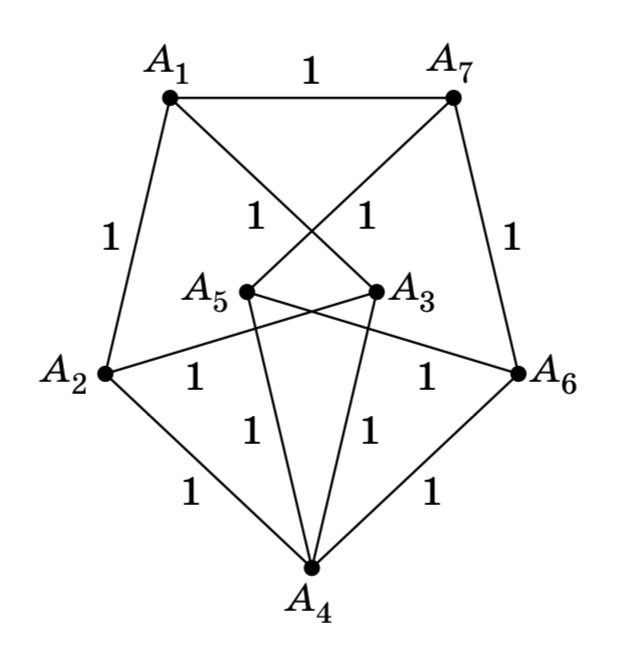
\includegraphics [width=0.8\linewidth] {Moser_Spindle}
  \caption{Веретено Мозера} 
  \label{img:latex}
\end{figure}

\begin{figure}[ht] 
  \center
  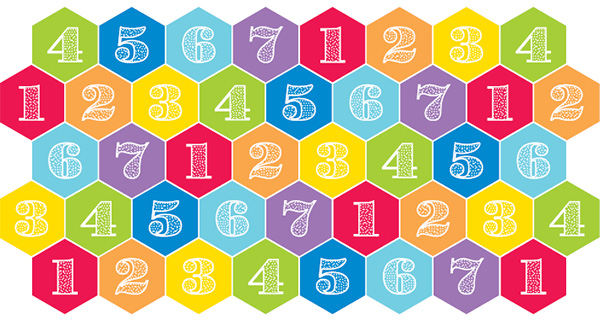
\includegraphics [width=0.8\linewidth] {raskraska7}
  \caption{Раскраска плоскости в 7 цветов} 
  \label{img:latex}
\end{figure}

В апреле 2018 года Обри де Грей опубликовал статью, в которой доказал, что хроматическое число плоскости хотя бы 5. На момент написания работы задача является открытой. Данная работа фокусируется на уточнении неясных мест в данной статье, явных детерминированных конструкциях графов из статьи и верификации отдельных утверждений статьи в системе Coq.

\section{Система Coq. Описание, история, возможности, применения}
История создания, история использования (сортировки, раскраска карты, \cite{} что-нибудь.)

Какая логика? Че за изоморфизм там? Что такое Галина? Мы пользуемся Галиной? Что такое тактики?

Мы будем пользоваться представлением графа чувака автора учебника, \cite{} учебник.

\section{Мотивировка задачи} \label{sect1_2}

Краткое изложение структуры статьи де Грея, статья просится на верификацию.


\section{Обзор литературы}

1. Huele
2. Exoo, Geoffrey; Ismailescu, Dan 

Пацаны проверили на SAT solver-e, кто-то придумал пример поменьше, кто-то графы по-другому делает.


\newcommand{\actuality}{}

%% регистрируем счётчики в системе totcounter
\regtotcounter{totalcount@figure}
\regtotcounter{totalcount@table}       % Если поставить в преамбуле то ошибка в числе таблиц
\regtotcounter{TotPages}               % Если поставить в преамбуле то ошибка в числе страниц

% \textbf{Объем и структура работы.} Работа состоит из~введения, трёх глав, заключения и~двух приложений.
%% на случай ошибок оставляю исходный кусок на месте, закомментированным
%Полный объём диссертации составляет  \ref*{TotPages}~страницу с~\totalfigures{}~рисунками и~\totaltables{}~таблицами. Список литературы содержит \total{citenum}~наименований.
%
% Полный объём работы составляет \formbytotal{TotPages}{страниц}{у}{ы}{} 
% с~\formbytotal{totalcount@figure}{рисунк}{ом}{ами}{ами}
% и~\formbytotal{totalcount@table}{таблиц}{ей}{ами}{ами}. Список литературы содержит  
% \formbytotal{citenum}{наименован}{ие}{ия}{ий}.
    % Введение
%\newpage
%============================================================================================================================


\chapter{Реализация графа в Coq}

\section{Представление графов в Coq}
Реализации графов из статьи де Грея приведены в файле {\tt myGraphs.v}~\ref{lst:myGraphs}
Эффективное представление графа было взято из\cite{VFA} и устроено
следующим образом: граф -- это конечное отображение, каждую вершину
(помеченную целым положительными числом) переводящее во
множество вершин с нею смежных. Конечные отображения и множества
формализованы с помощью модулей FSets и FMaps из стандартной
библиотеки. Эти модули принимают различные типы ключей, в данном случае мы будем использовать тип {\tt positive} целых положительных чисел в двоичном представлении из модуля {\tt PositiveOrderedTypeBits}.

\begin{verbatim}
Module E := PositiveOrderedTypeBits.
Module S <: FSetInterface.S := PositiveSet.
Module M <: FMapInterface.S := PositiveMap.
\end{verbatim} 

Вершина {\tt node} -- это элемент типа {\tt positive}, {\tt nodemap} -- это отображение из вершин, а граф {\tt graph} -- это отображение из типа вершина в тип множество вершин. Тип {\tt positive} был выбран из-за того, что в нем оператор сравнения определен так, чтобы поиск по ключу типа {\tt positive} в множестве и отображении был более эффективным.

\begin{verbatim}
Definition node := E.t.
Definition nodeset := S.t.
Definition nodemap: Type -> Type := M.t.
Definition graph := nodemap nodeset.
\end{verbatim}

Для работы с графами были определены функции добавления ребра в существующий граф и построения графа из списка ребер.

\begin{verbatim}
Definition add_edge (e: (E.t*E.t)) (g: graph) : graph :=
 M.add (fst e) (S.add (snd e) (adj g (fst e))) 
  (M.add (snd e) (S.add (fst e) (adj g (snd e))) g).
\end{verbatim}

В данной функции ребро представляется парой вершин.
В данной работе реализуются неориентированные графы без петель.

\begin{verbatim}
Definition mk_graph (el: list (E.t*E.t)) :=
  fold_right add_edge (M.empty _) el.
\end{verbatim}

В терминах определенных выше функций построение графа {\tt K3} выглядит следующим образом:
\begin{verbatim}
Definition K3 := 
    mk_graph [ (1, 2) ; (2, 3); (1, 3)].
\end{verbatim}

Далее для работы с графом можно использовать функцию вывода множества вершин и функцию {\tt gr\_show} вывода множества ребер.
\begin{verbatim}
Compute (S.elements (Mdomain K3)).
\end{verbatim}
{\it = [2; 1; 3]}

{\it    : list S.elt.}

\begin{verbatim}
Function gr_show (g : graph) : list (node * node) :=
  S.fold 
    (fun n l => (map (fun y => (n, y)) (S.elements (adj g n))) ++ l) 
    (Mdomain g) nil.
\end{verbatim}

\begin{verbatim}
Compute gr_show K3.
\end{verbatim}
{\it = [(3, 2); (3, 1); (1, 2); (1, 3); (2, 1); (2, 3)] }

{\it   : list (node * node) }

В статье \cite{deGrey} автор приводит граф единичных расстояний {\tt N}, который раскрашивается в 4 цвета. Этот граф строится поэтапно на основании других графов. Сначала автор рассматривает граф $$H := (\{1, 2, 3, 4, 5, 6, 7 \},$$
    $$ \{(1, 2), (1, 3), (1, 4), (1, 5), (1, 6), (1, 7), $$
    $$ (2, 3), (3, 4), (4, 5), (5, 6), (6, 7), (7, 2)\}) $$ и замечает, что существет 4 существенно различных способа правильно раскрасить граф {\tt H} в не более чем 4 цвета.
    
Далее автор поэтапно, через графы {\tt H}, {\tt J} и {\tt K}, строит граф {\tt L} и рассматривает его правильные раскраски.

Конструкции графов в работе де Грея обладают
высокой степенью симметрии. Мы разработали и частично верифицировали в
системе {\tt Coq} методы построения таких графов. Именно, мы реализуем
функцию {\tt mk\_art}, которая соединяет два графа по вершине, {\tt mk\_cmn\_edge}, которая соединяет два графа по ребру и {\tt add\_edges}, которая добавляет ребра в граф.

Для реализации этих функций потребовались следующие вспомогательные функции.
Рекурсивная функция {\tt l\_rng} находит минимум и максимум в списке, функция {\tt gr\_rng} находит в графе минимальный и максимальный номера вершин. Функция {\tt rename\_all} принимает на вход граф {\tt G} и функцию {\tt f} из номеров вершин в номера вершин и выдает граф, полученный применением {\tt f} к вершинам графа {\tt G}. Функция {\tt delete\_edge} удаляет ребро из графа, а функция {\tt rename\_in\_order} переименовывает вершины графа в отрезок от $1$ до количества вершин, сохраняя при этом их порядок.


В терминах описанных функций конструкция графа {\tt H} на основе графа {\tt K3} выглядит следующим образом:

\begin{verbatim}
Definition H : graph := 
  let g1 := rename_in_order (mk_cmn_edge K3 K3 1 3 1 3) in
  let g2 := rename_in_order 
                (mk_cmn_edge g1 K3 1 (snd (gr_rng g1)) 1 3) in
  let g3 := rename_in_order 
                (mk_cmn_edge g2 K3 1 (snd (gr_rng g2)) 1 3) in
  let g4 := rename_in_order 
                (mk_cmn_edge g3 K3 1 (snd (gr_rng g3)) 1 3) in
  rename_in_order (add_edge (2, snd (gr_rng g4)) g4).
\end{verbatim}

Т.~е. граф {\tt H} построен из $5$ копий {\tt K3}, склеенных друг с другом по ребру, и добавленного ребра.

\begin{figure}[ht] 
  \center
  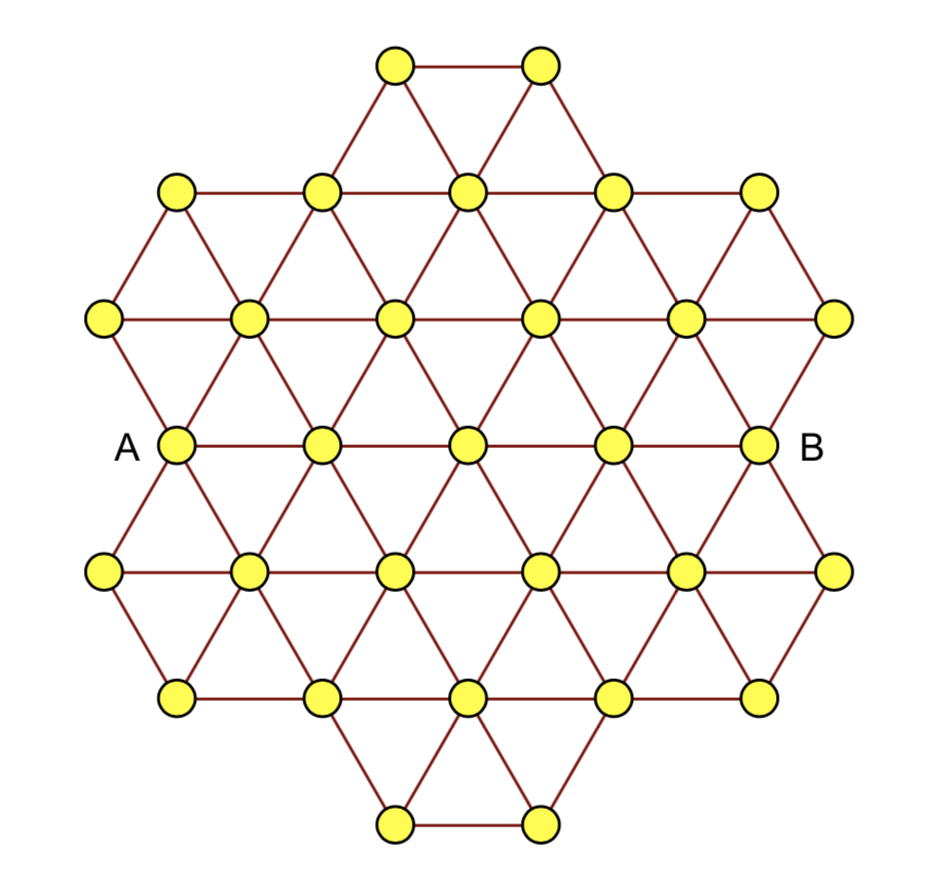
\includegraphics [width=0.5\linewidth] {Graph_J}
  \caption{Граф J} 
  \label{img:Graph_J}
\end{figure}

Граф {\tt J} состоит их 6 копий {\tt H}, склеенных между собой по ребру.
\begin{verbatim}
Definition J: graph :=
  let HH := mk_cmn_edge H H 2 3 6 7 in
  let HH_H := mk_cmn_edge HH H 7 2 6 7 in
  let HHH := rename_node 14 12 HH_H in
  let HHH_H := mk_cmn_edge HHH H 6 7 6 7 in
  let HHHH := rename_node 19 17 HHH_H in
  let HHHH_H := mk_cmn_edge HHHH H 5 6 6 7 in
  let HHHHH := rename_node 24 22 HHHH_H in
  let HHHHH_H := mk_cmn_edge HHHHH H 4 5 6 7 in
  let HHHHHH := rename_node 29 27 HHHHH_H in
  let HHHHHH_H := mk_cmn_edge HHHHHH H 3 4 6 7 in
  let HHHHHHH :=  rename_node 34 32 HHHHHH_H in
  rename_in_order (rename_node 37 9 HHHHHHH).
\end{verbatim}

В графе {\tt J} вершины, находящиеся на расстоянии $2$ от центра (в данной реализации вершины 9, 12, 16, 20, 24, 28) называются {\it соединяющими вершинами}.

\begin{figure}[ht] 
  \center
  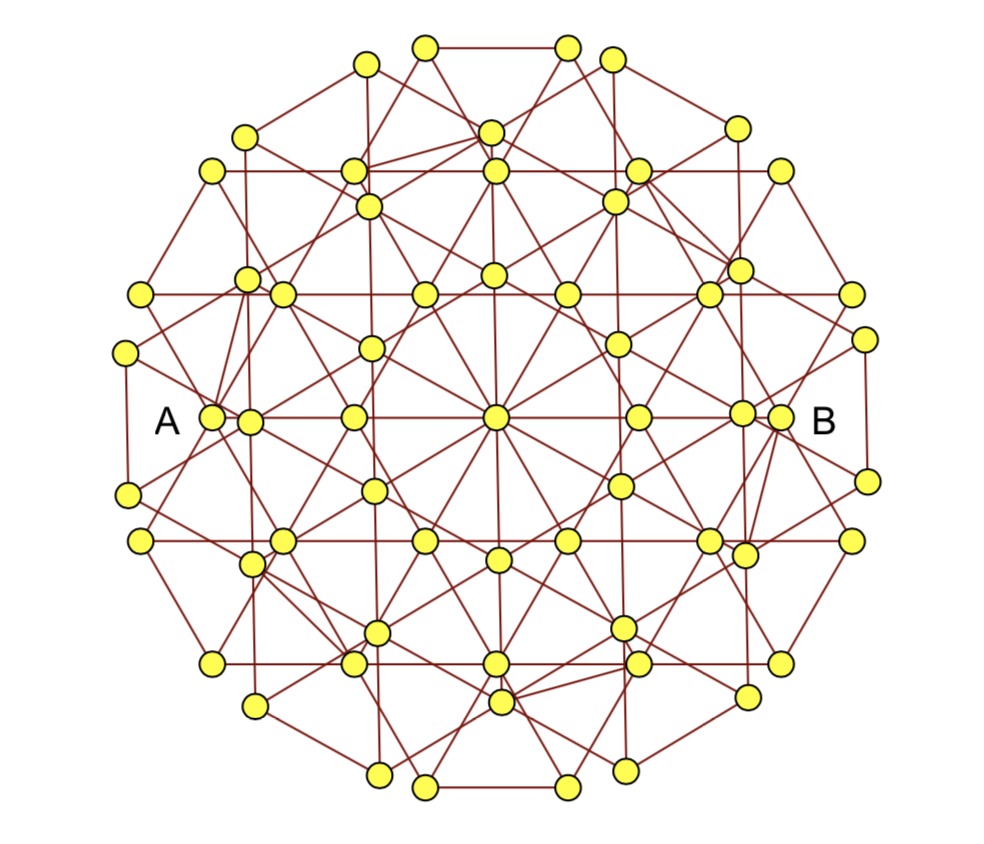
\includegraphics [width=0.8\linewidth] {Graph_K}
  \caption{Граф K} 
  \label{img:Graph_K}
\end{figure}

Граф {\tt K} состоит из двух копий графа {\tt J}, соединенных по центру, и ребер между соответствующими {\it соединяющими вершинами}.

\begin{verbatim}
Definition K: graph :=
  let JJ := mk_art J J 1 1 in
  let JJ := add_edges [
            (9, 9+31); (12, 12+31); (16, 16+31);
            (20, 20+31); (24, 24+31); (28, 28+31)] JJ in
  rename_in_order JJ.
\end{verbatim}

Наконец, граф {\tt L} состоит из двух копий графа {\tt K}, склееных между собой по {\it соединяющей вершине} и ребра между соединяющими вершинами, являющимися противоположными точке соединения.

\begin{figure}[ht] 
  \center
  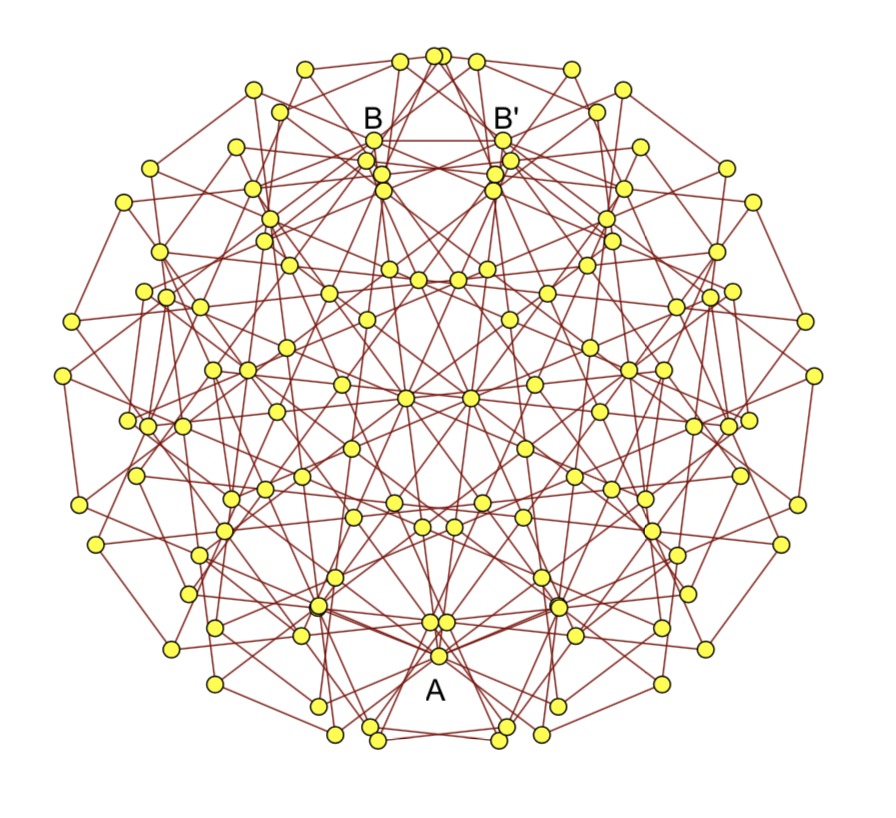
\includegraphics [width=0.8\linewidth] {Graph_L}
  \caption{Граф L} 
  \label{img:Graph_L}
\end{figure}

\section{Доказательства корректности операций над графами}

В файле {\tt myGraphs\_Properties.v}~\ref{lst:myGraphs_Properties} представлены доказательства корректности отпределенных ранее графов, т.~е. что они являются неориентированными графами без петель. 

\begin {verbatim}
Definition graph_ok (g : graph) := 
  undirected g /\ no_selfloop g.
\end{verbatim}

Для доказательства корректности графов введены и доказаны вспомогательные леммы {\tt adj\_M\_In} и {\tt edge\_corr\_1}.

\begin {verbatim}
Lemma adj_M_In : forall g n m,
  S.In m (adj g n) -> M.In n g.
\end{verbatim}

\begin {verbatim}
Lemma edge_corr_1 : forall g n m, edge g n m -> S.In m (nodes g).
\end{verbatim}

А также определена тактика {\tt gr\_destr}.

\begin {verbatim}
Ltac gr_destr h :=   apply S.elements_1 in h; compute in h;
  repeat rewrite InA_cons in h; rewrite InA_nil in h;
  repeat destruct h as [? | h]; try inversion h; subst.
\end{verbatim}

Данная тактика из посылки, что {\tt i} -- вершина графа, заключает, что {\tt i} равняется какому-то числу от $1$ до количества вершин и использует инверсию на этой посылке, тем самым перебирая все возможные вершины графа.

С использованием этой тактики доказательство корректности выглядит одинаково для любого построенного выше графа, приведем его для {\tt H}:

\begin{verbatim}
Lemma H_ok : graph_ok H.
Proof.
split.
- unfold undirected. intros. remember H as H'.
  clear HeqH'. apply edge_corr_1 in H.
  gr_destr H; gr_destr H';  reflexivity.
- unfold no_selfloop. repeat intro. remember H as H'.
  clear HeqH'. apply edge_corr_1 in H. gr_destr H; gr_destr H';
  discriminate.
Qed.
\end{verbatim}

Наряду с непосредственной проверкой корректности графов, можно доказать сохранение свойств отсутствия ориентации и петель нашими функциями, привлекаемыми для их построения (такими как {\tt add\_edge} и пр.). Очевидно, такой подход более универсален и более эффективен, поскольку, например уже для графа {\tt J} верификация доказательства занимает существенное время:

\begin{verbatim}
Lemma J_ok : graph_ok J.
Proof.
split.
- unfold undirected. intros. remember H as H'.
  clear HeqH'. apply edge_corr_1 in H.
  gr_destr H; gr_destr H';  reflexivity.
- unfold no_selfloop. repeat intro. remember H as H'.
  clear HeqH'. apply edge_corr_1 in H. gr_destr H; gr_destr H';
  discriminate.
Time Qed.
\end{verbatim}

{\it J\_ok is defined}

{\it Finished transaction in 73.252 secs (67.009u,0.208s) (successful) }

Мы приводим доказательство теоремы 

\begin{verbatim}
Lemma add_edge_corr : forall g a b, graph_ok g -> a <> b -> 
  graph_ok (add_edge (a, b) g).
\end{verbatim}
в файле {\tt myGraphs\_Properties.v}. Оно опирается на лемму 

\begin{verbatim}
Lemma add_edge_corr' : forall g x y a b,
  edge (add_edge (a, b) g) x y <-> edge g x y \/ (x = a /\ y = b) \/ 
  (x = b /\ y = a).
\end{verbatim}

дающую спецификацию функции {\tt add\_edge} и доказываемую с помощью принципа индукции {\tt WP.map\_induction} для конечных отображений из стандартной библиотеки.

\chapter{Доказательство свойств раскраски малых графов в Coq}
Назовем две раскраски $f$, $f'$ графа $G$ {\it существенно одинаковыми}, если существуют изоморфизм графа $g$ и перестановка цветов $ \omega $ такие, что
$f(v) = \omega ( f'( g(v) ) )$ . Также назовем две раскраски {\it существенно различными}, если они не являются существенно одинаковыми.

{\it Граф H} -- это граф $$H := (\{1, 2, 3, 4, 5, 6, 7 \},$$
    $$ \{(1, 2), (1, 3), (1, 4), (1, 5), (1, 6), (1, 7), $$
    $$ (2, 3), (3, 4), (4, 5), (5, 6), (6, 7), (7, 2)\}) $$
    

\begin{figure}[ht] 
  \center
  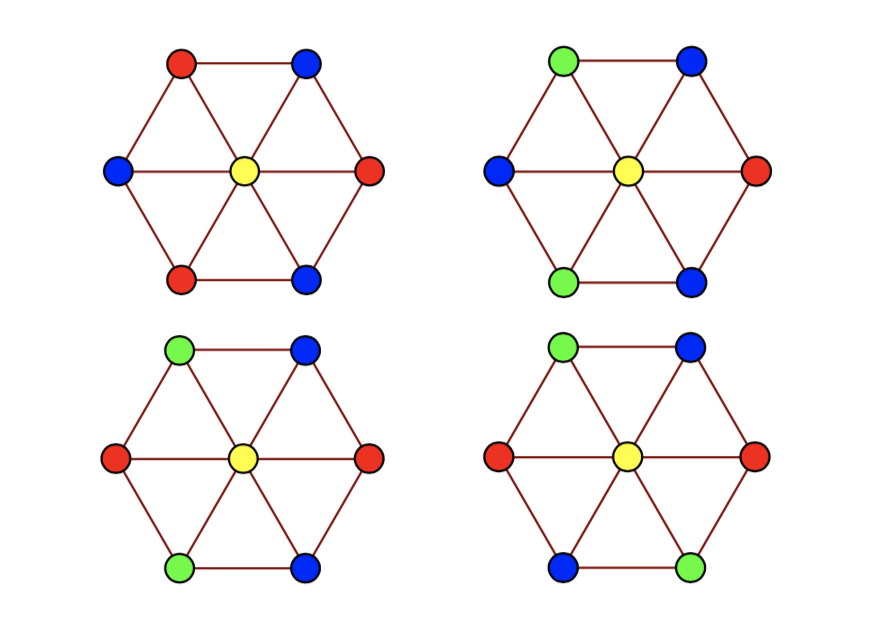
\includegraphics [width=0.8\linewidth] {Colorings_of_H}
  \caption{Существенно различные способы раскрасить граф H в не более чем 4 цвета} 
  \label{img:Colorings_of_H}
\end{figure}

В статье \cite{deGrey} утверждается что существует только 4 существенно различные раскраски графа {\tt H} в не более чем в 4 цвета. Это утверждение обосновывается перебором вариантов наличия или отсутствия монохроматических троек.

Описание типов для работы с раскрасками находятся в файле {\tt my\_New\_Coloring.v}~\ref{lst:my_New_Coloring}. В нем описан индуктивный предикат {\tt is\_color}, где {\tt is\_color} означает, что номер цвета содержится в палитре из 4 цветов. Тот факт, что этот тип индуктивный, позволяет использовать тактику {\tt inversion}, перебирая разрешенные цвета.

\section{Язык {\tt Ltac}, {\tt pattern matching} и {\tt goal matching} }
В данной главе активно используется язык {\tt Ltac} и инструмент {\tt goal matching}, представляемый этим языком.
Язык {\tt Ltac}, впервые представленный в статье <<A Tactic Language for the System {\tt Coq}>>~\cite{Del00}, предоставляет оператор соответствия ({\tt pattern matching}) не только для термов, но и для контекста доказательства ({\tt goal matching}), т.~е. цели и посылок. Данный оператор позволяет автоматизировать применение низкоуровневых тактик и значительно сократить длину доказательства.

\section{Типы возможных правильных раскрасок графа {\tt T} в не более чем 4 цвета}

Назовем {\it тройкой} любой граф, изоморфный графу {\it T} на четырех вершинах $$T = (\{1, 2, 3, 4\} , \{(1, 2), (1, 3), (1, 4) \} ).$$

{\it Утверждение}: Существует только три существенно различные раскраски графа $G$, если граф $G$ изоморфен $T$.

Код доказательства этого утверждения приведен в файле {\tt my\_Triple\_Coloring.v}~\ref{lst:my_Triple_Coloring}. 

В системе {\tt Coq} эти раскраски можно описать следующим образом:

\begin{verbatim}
(* Monochromatic *)
Definition type1_triple (el: list node) (c: Coloring) :=
  let center := nth 0 el 1 in
  let v1 := nth 1 el 1 in
  let v2 := nth 2 el 1 in
  let v3 := nth 3 el 1 in
  let c1 := c center in
  let c2 := c v1 in
  ~ (c1 = c2) /\ same_color c v1 v2 /\ same_color c v2 v3.

(* 2 and 1 *)
Definition type2_triple (el: list node) (c: Coloring) :=
  let center := nth 0 el 1 in
  let v1 := nth 1 el 1 in
  let v2 := nth 2 el 1 in
  let v3 := nth 3 el 1 in

  let c1 := c center in
  let c2 := c v1 in
  let c3 := c v2 in 
  let c4 := c v3 in
  ~ (c1 = c2) /\ ~ (c1 = c3) /\ ~ (c1 = c4) /\
    ( (c2 = c3 /\ ~ c2 = c4) \/ (c2 = c4 /\ ~ c2 = c3) \/ 
        (c3 = c4 /\ ~ c3 = c2) ).

(* All 3 different *)
Definition type3_triple (el: list node) (c: Coloring) :=
  let center := nth 0 el 1 in
  let v1 := nth 1 el 1 in
  let v2 := nth 2 el 1 in
  let v3 := nth 3 el 1 in

  let c1 := c center in
  let c2 := c v1 in
  let c3 := c v2 in 
  let c4 := c v3 in
  ~ (c1 = c2) /\ ~ (c1 = c3) /\ ~ (c1 = c4) /\
    (~ c2 = c3) /\ (~ c2 = c4) /\ (~ c3 = c4).
\end{verbatim}

Каждый предикат принимает на вход список вершин и раскраску, при этом первый элемент в списке -- номер вершины, соединенной со всеми остальными. Предикат {\tt type1\_triple} кодирует то, что все вершины, кроме первой одинакового цвета, при этом этот цвет отличен от цвета первой вершины. Предикат {\tt type2\_triple} кодирует то, что цвет первой вершины отличен от цвета остальных вершин, а среди остальных есть две одинакового цвета, который отличен от цвета оставшейся вершины. Предикат {\tt type3\_triple} кодирует случай, когда все 4 вершины имеют различный цвет.

Теорема {\tt coloring\_triple\_T} утверждает, что любая правильная раскраска графа {\tt T} является раскраской одного из этих типов. Ее доказательство включает в себя перебор всех возможных раскрасок, однако благодаря использованию языка {\tt Ltac} и {\tt goal matching} можно переиспользовать куски доказательства в ситуациях, отличающихся только перестановкой цветов или изоморфизма графа.

Тактика {\tt contr} доказывает {\tt coloring\_triple\_T} от противного и применяется в случаях, когда раскраска не является правильной, т.~е. существует пара смежных ребер одного цвета. Тактика {\tt type1\_tac} применяется, когда полученная раскраска является раскраской первого типа, тактики {\tt type1\_tac\_left}, {\tt type1\_tac\_middle}, {\tt type1\_tac\_right} -- раскраской второго типа (какая именно тактика будет применена зависит от того, какая пара вершин окрашена в один цвет) и тактика {\tt type3\_tac} применяется для доказательства того, что раскраска является раскраской третьего типа.

Таким образом, для любой раскраски графа {\tt T} существует тактика, с помощью которой можно доказать утверждение о том, что если раскраска правильная, то она является раскраской одного из трех типов. Теперь все эти тактики можно объединить в одну тактику {\tt level4}, которая с помощью {\tt goal matching} может определить, какую именно тактику из указанных использовать. Теперь можно создать тактики {\tt level3} и {\tt level2}, которые также с помощью {\tt goal matching} определяют, необходимо ли доказывать утверждение от противного или вызывать тактику следующего уровня.

Итак, благодаря {\tt goal matching} доказательство утверждения при различных контестах может быть доказано одной и той же тактикой, что позволяет использовать конвейер и записать доказательство теоремы очень кратко

\begin{verbatim}
Lemma coloring_triple_T:
  forall c: Coloring, is_good_coloring c T ->
  type1_triple [1; 2; 3; 4] c \/ type2_triple [1; 2; 3; 4] c \/
  type3_triple [1; 2; 3; 4] c.
Proof.
  intros. unfold is_good_coloring in H. unfold is_coloring in H. 
  destruct H. remember H as H'. clear HeqH'. 
  specialize (H' 1). inversion H';
    remember H as H''; clear HeqH''; specialize (H'' 2); 
    inversion H''; remember H0 as H0'; clear HeqH0';
      level2 H H0' H0 H2 H3 c.
Qed.
\end{verbatim}

\section{Типы возможных правильных раскрасок графа {\tt H} в не более чем 4 цвета}

Теперь, когда доказано утверждение про правильные раскраски {\it троек}, можно перейти к раскраскам графа {\it H}.

Типы раскрасок графа {\it H} в не более чем 4 цвета можно описать следующими предикатами в системе {\tt Coq}.

\begin{verbatim}
(* Type1 triple - Type1 triple *)
Definition type1_H (c: Coloring) : Prop :=
  type1_triple [1; 2; 4; 6] c /\ type1_triple [1; 3; 5; 7] c /\
    ~ same_color c 2 3.

(* Type1 triple - Type2 triple *)
Definition type2_H (c: Coloring) : Prop :=
  (type1_triple [1; 2; 4; 6] c /\ type2_triple [1; 3; 5; 7] c /\
    ~ same_color c 2 3 /\ ~ same_color c 2 5 /\ ~ same_color c 2 7) \/
  (type2_triple [1; 2; 4; 6] c /\ type1_triple [1; 3; 5; 7] c /\
    ~ same_color c 2 3 /\ ~ same_color c 4 3 /\ ~ same_color c 6 3).

(* Diagonals are monochromatic *)
Definition type3_H (c: Coloring) : Prop :=
  type3_triple [1; 2; 4; 6] c /\ type3_triple [1; 3; 5; 7] c /\
    same_color c 2 5 /\ same_color c 3 6 /\ same_color c 4 7.

(* One monochromatic diagonal and 
same colors close to the vertices in diagonal *)
Definition type4_H (c: Coloring) : Prop :=
  type2_triple [1; 2; 4; 6] c /\ type2_triple [1; 3; 5; 7] c /\
  (
    (* Diagonal is 2 5 *) 
    (same_color c 2 5 /\ same_color c 3 7 /\ same_color c 4 6 ) \/

    (* Diagonal is 3 6 *) 
    (same_color c 3 6 /\ same_color c 2 4 /\ same_color c 5 7 ) \/

    (* Diagonal is 4 7 *) 
    (same_color c 4 7 /\ same_color c 3 5 /\ same_color c 2 6 )
  ).
\end{verbatim}

В системе {\tt Coq} теорема о возможных раскрасках графа {\tt H} формулируется следующим образом:

\begin{verbatim}
Lemma coloring_H:
  forall c: Coloring, is_good_coloring c H ->
  type1_H c \/ type2_H c \/ type3_H c \/ type4_H c.
\end{verbatim}

Полный код доказательства находится в файле {\tt my\_H\_Coloring.v}~\ref{lst:my_H_coloring}.

Как и в предыдущем разделе, можно определить тактику {\tt contr}, которая доказывает утверждение от противного, т.~е. доказывает, что данная раскраска не является правильной. Но так как теперь вершин в графе больше и не всегда понятно, какие именно смежные вершины окрашены в одинаковый цвет, доказательство упрощает использование тактики {\tt find\_contr}, которая перебирает гипотезы-посылки о том, что какие-то две вершины покрашены в один цвет в контексте доказательства и пытается из этих гипотез вывести, что раскраска не является правильной. 

Также определены тактики 

{\tt type1\_H\_tac}, {\tt type2\_H\_tac\_left\_left}, {\tt type2\_H\_tac\_left\_right}, {\tt type2\_H\_tac\_left\_middle}, {\tt type2\_H\_tac\_right\_left}, {\tt type2\_H\_tac\_right\_middle}, {\tt type2\_H\_tac\_right\_right}, {\tt type3\_H\_tac}, {\tt type4\_H\_tac\_1}, {\tt type4\_H\_tac\_2}, {\tt type4\_H\_tac\_3} для каждого подтипа раскраски. Для автоматизации использования этих тактик разработана еще одна тактика {\tt find\_type}, в которой используется оператор соответствия цели ({\tt goal matching}). Тактика {\tt color\_next} <<окрашивает следующую вершину>>, т.~е. выводит посылку о том, что цвет следующей вершины принадлежит индуктивному типу {\tt is\_color} и делает инверсию этого типа.

Итоговое доказательство теоремы выглядит следующим образом:

\begin{verbatim}
Lemma coloring_H:
  forall c: Coloring, is_good_coloring c H ->
  type1_H c \/ type2_H c \/ type3_H c \/ type4_H c.
Proof.
  intros. unfold is_good_coloring in H. 
  unfold is_coloring in H. destruct H.
  color_next H 1;
    color_next H 2; try find_contr H0 c;
      color_next H 3; try find_contr H0 c;
        color_next H 4; try find_contr H0 c;
          color_next H 5; try find_contr H0 c;
            color_next H 6; try find_contr H0 c;
              color_next H 7; try find_contr H0 c;
                find_type H3 H5 H7 H9 H11 H13 H15 c.
Qed.
\end{verbatim}

\chapter{Работа в графами на {\tt Python}}
\section{Реализация графов на плоскости}
Все встречавшиеся ранее графы являются {\it графами единичных расстояний}, т.~е. существует такая реализация этих графов на плоскости, в которой каждое ребро имеет длину 1.

Работа с реализацией графа на плоскости в системе {\tt Coq} представляет затруднения, так как формализация представления и разработка операций над алгебраическими числами влечет за собой большую работу.

Чтобы получить реализацию графов на плоскости, использовался язык {\tt Python} и пакет для символьной математики {\tt Sympy}.

Код для генерации реализаций рассматриваемых графов на плоскости находится в файле {\tt SymPy\_Realization.py}.

Для работы с реализациями графов были определены следующие функции. Функция {\tt neg(pt)} отражает вектор {\tt pt} относительно начала координат, функция {\tt shifted(pt, vec)} сдвигает вектор {\tt pt} на вектор {\tt vec}, функция {\tt rotated(pt, angle)} поворачивает вектор {\tt pt} на угол {\tt angle} относительно начала координа, функция {\tt rotatedabout(pt, origin, angle)} поворачивает вектор {\tt pt} на угол {\tt angle} относительно точки {\tt origin}.

Генерация реализаций на плоскости графов {\tt H} и {\tt J} выглядят следующим образом:

\begin{verbatim}
def build_H():
    o = (Rational(0), Rational(0))
    e = (Rational(1), Rational(0))

    H = {o}
    for i in range(6):
        H.add(rotatedabout(e, o, pi / 3 * i))
    H = simplified(H)
    return H
\end{verbatim}

\begin{verbatim}
def build_J():
    J = {o}
    for i in range(6):
        J.update(
            { rotated(
                shifted(x, shifted(
                            e, rotated(e, pi / 3)
                                  ) 
                        ),
                pi / 3 * i) for x in H }
                )
    return simplified(J)
\end{verbatim}

Остальные графы вплоть до {\tt L} генерируются, как указано в статье~\cite{deGrey}.
% def dist2(p, q):
% def simplified(pts):
% def factored(pts):
% def check_zero(x):

\section{Алгоритм раскраски графов}
Одна из подзадач статьи~\cite{deGrey} заключается в том, чтобы найти такой граф {\tt M}, содержащий копию {\tt H}, что ни при какой правильной раскраске графа {\tt M} содержащаяся копия {\tt H} не содержит граф T', изоморфный T, раскрашенный по типу 1 (все три висячие вершины одного цвета).
В разделе 4 статьи~\cite{deGrey} предложен алгоритм для проверки графов на обладание указанным свойством.

Алгоритм обходит граф в глубину и красит встречающиеся вершины в первый доступный цвет. Если на каком-то шаге алгоритма есть вершина, для которой никакой цвет не является доступным, происходит {\it возврат} ({\tt backtracking}). А если на каком-то шаге есть вершины, для которых доступен только один цвет, то красятся эти вершины. Полный код алгоритма представлен в файле {\tt Color\_graph-M.py}.


\chapter{Заключение}
\section{Выводы}
В статье ~\cite{deGrey} представлен граф единичных расстояний {\tt N}, который не красится в 4 цвета. Этот граф представляет собой прямое произведение графов {\tt L} и {\tt M}.

В данной работе представлены эффективные методы конструирования графов, обладающих высокой степенью симметрии. Эти методы были применены к графам {\tt H}, {\tt J}, {\tt K} и {\tt L}.

Также разработаны методы работы с раскрасками графов и методики верифицирования доказательств теорем о свойствах раскрасок. Верифицировано доказательство того, что существует ровно 4 существенно различных раскрасок графа {\tt H}. Разработанные методы можно использовать и для других графов.

Графы из второй части статьи ~\cite{deGrey} реализованы не были в силу того, что их конструкция сильно опирается на реализацию этиз графов на плоскости. В то же время, был реализован на Python алгоритм из второй части статьи, с помощью которого производился поиск подходящего графа {\tt M}.

\section{Планы будущей работы}
Разработанные методы конструкции графов, обладающих высокой степенью симметрии, можно использовать для графов из статьи Marijn~J.H.~Heule, <<Computing Small Unit-Distance Graphs with Chromatic Number 5>>~\cite{Huele}, в которой приводится граф меньшего размера, который не красится в 4 цвета.

Методы работы в системе {\tt Coq} с раскрасками графов можно применить для доказательства свойств раскраски графов {\tt J}, {\tt K} и {\tt L}.

Также интерес представляет верифицирование с помощью {\Coq} алгоритма покраски графа из статьи~\cite{deGrey}, с помощью которого был осуществлен поиск графа, подходящего на роль {\tt M}.

\chapter{Приложение}

\begingroup
    \lstinputlisting[caption={Листинг myGraphs.v},label={lst:myGraphs}]{listings/myGraphs.v}
\endgroup
 
\begingroup
    \lstinputlisting[caption={Листинг myGraphs\_Properties.v},label={lst:myGraphs_Properties}]{listings/myGraphs_Properties.v}
\endgroup

\begingroup
    \lstinputlisting[caption={Листинг my\_New\_Coloring.v},label={lst:my_New_Coloring}]{listings/my_New_Coloring.v}
\endgroup


\begingroup
    \lstinputlisting[caption={Листинг my\_Triple\_Coloring.v},label={lst:my_Triple_Coloring}]{listings/my_Triple_Coloring.v}
\endgroup


\begingroup
    \lstinputlisting[caption={Листинг my\_H\_coloring.v},label={lst:my_H_coloring}]{listings/my_H_coloring.v}
\endgroup
 
\begingroup
    \lstinputlisting[caption={Листинг Color\_graph-M.py},label={lst:Color_graph-M},language={python}]{listings/Color_graph-M.py}
\endgroup
   
\begingroup
    \lstinputlisting[caption={Листинг SymPy\_Realization.py},label={lst:SymPy_Realization},language={python}]{listings/SymPy_Realization.py}
\endgroup

\label{chapt1}
           % Глава 1
% \input{conclusion}      % Заключение
\begin{thebibliography}{0}
    
    \bibitem{deGrey}
    A.~de~Grey, 
    The chromatic number of the plane is at least 5, 
    {\it \href{arXiv:1804.02385}{arXiv:1804.02385}, }
    --- 2018. 
    
    \bibitem{VFA}
    Andrew~W.~Appel, 
    Software Foundations, Volume 3: Verified Functional Algorithms, 
    {\it \href{https://softwarefoundations.cis.upenn.edu/vfa-current/}{https://softwarefoundations.cis.upenn.edu/vfa-current/}, }
    --- 2017. 


    \bibitem{Had}
    H.~Hadwiger,
    Ueberdeckung des Euklidischen Raumes durch kongruente Mengen,
    {\it Portugaliae mathematica,}
    4(4), 238-242 (1945).
    
    \bibitem{Soi}
    A.~Soifer,
    {\it The Mathematical Coloring Book,}
    Springfer, 2008, ISBN-13: 9780387746401.

    \bibitem{Huele}
    Marijn~J.H.~Heule,
    Computing Small Unit-Distance Graphs with Chromatic Number 5,
    {\it \href{ arXiv:1805.12181}{ arXiv:1805.12181 },} 
    --- 2018.
    
    \bibitem{NewProof}
    G.~Exoo, D.~Ismailescu,
    The chromatic number of the plane is at least 5 --- a new proof,
    {\it \href{ arXiv:1805.00157}{ arXiv:1805.00157}, }
    --- 2018.
    

\end{thebibliography}      % Список литературы
% \clearpage
\phantomsection
\addcontentsline{toc}{chapter}{\listfigurename}
\listoffigures									% Список изображений


%%% Список таблиц %%%
% (ГОСТ Р 7.0.11-2011, 5.3.10)
\clearpage
\phantomsection
\addcontentsline{toc}{chapter}{\listtablename}
\listoftables									% Список таблиц
\newpage           % Списки таблиц и изображений (иллюстративный материал)
% \input{appendix}        % Приложения

\end{document}
